\begin{frame}
\frametitle{A Formal Framework for HP Transfer}
\vspace{2mm}

\begin{block}{Definition: Convergent Quantities}

\begin{itemize}\setlength\itemsep{0.2em}
    \item[\ding{112}] \colorbox{teal!12}{\textbf{Loss (performance) gap:}} $a_n = |\phi_n^* - \phi_\infty^*|$. 
    \visible<2->{\item[\ding{112}]  \colorbox{teal!12}{\textbf{Hyperparameter gap:}} $b_n = \norm{\vnu_n^* - \vnu_\infty^*}$.}
    \visible<3->{\item[\ding{112}] \colorbox{FlatironOrange2!15}{\textbf{Transfer suboptimality gap:}} $c_n = |\phi_\infty(\vnu_n^*) - \phi_\infty(\vnu_\infty^*)|$.} 
\end{itemize}
    
\end{block}

\vspace{1mm}

\begin{columns}[T,onlytextwidth]
  % Left column
\begin{column}{0.54\textwidth}
\vspace{-1.5mm}

\small
\begin{itemize}\setlength\itemsep{0.15em}  \color{lightgray!60!black} 
    \item {\color{red!75!black}$a_n$} tracks how fast the loss (at optimal HP) converges with scale. 
    \visible<2->{\item {\color{red!75!black}$b_n$} tracks how fast the optimal HP converges with scale.} 
    \visible<3->{\item {\color{red!75!black}$c_n$} \color{black}  tracks convergence of the {\color{FlatironOrange2!90!black}\textit{transfer}} strategy, i.e., training a large model $n\to\infty$ with finite-$n$ optimal HP.} 
\end{itemize}

    \visible<4->{%

    \vspace{-5mm}
      \normalsize
      \begin{minipage}[t]{0.94\linewidth} \begin{block}{} 
      \centering
      \textbf{Question:} How do $a_n,b_n,c_n$ relate? 
      \end{block} \end{minipage}
    }
\end{column}

  % Right column
  \begin{column}{0.46\textwidth}
    \only<1|handout:0>{%
      \centering
      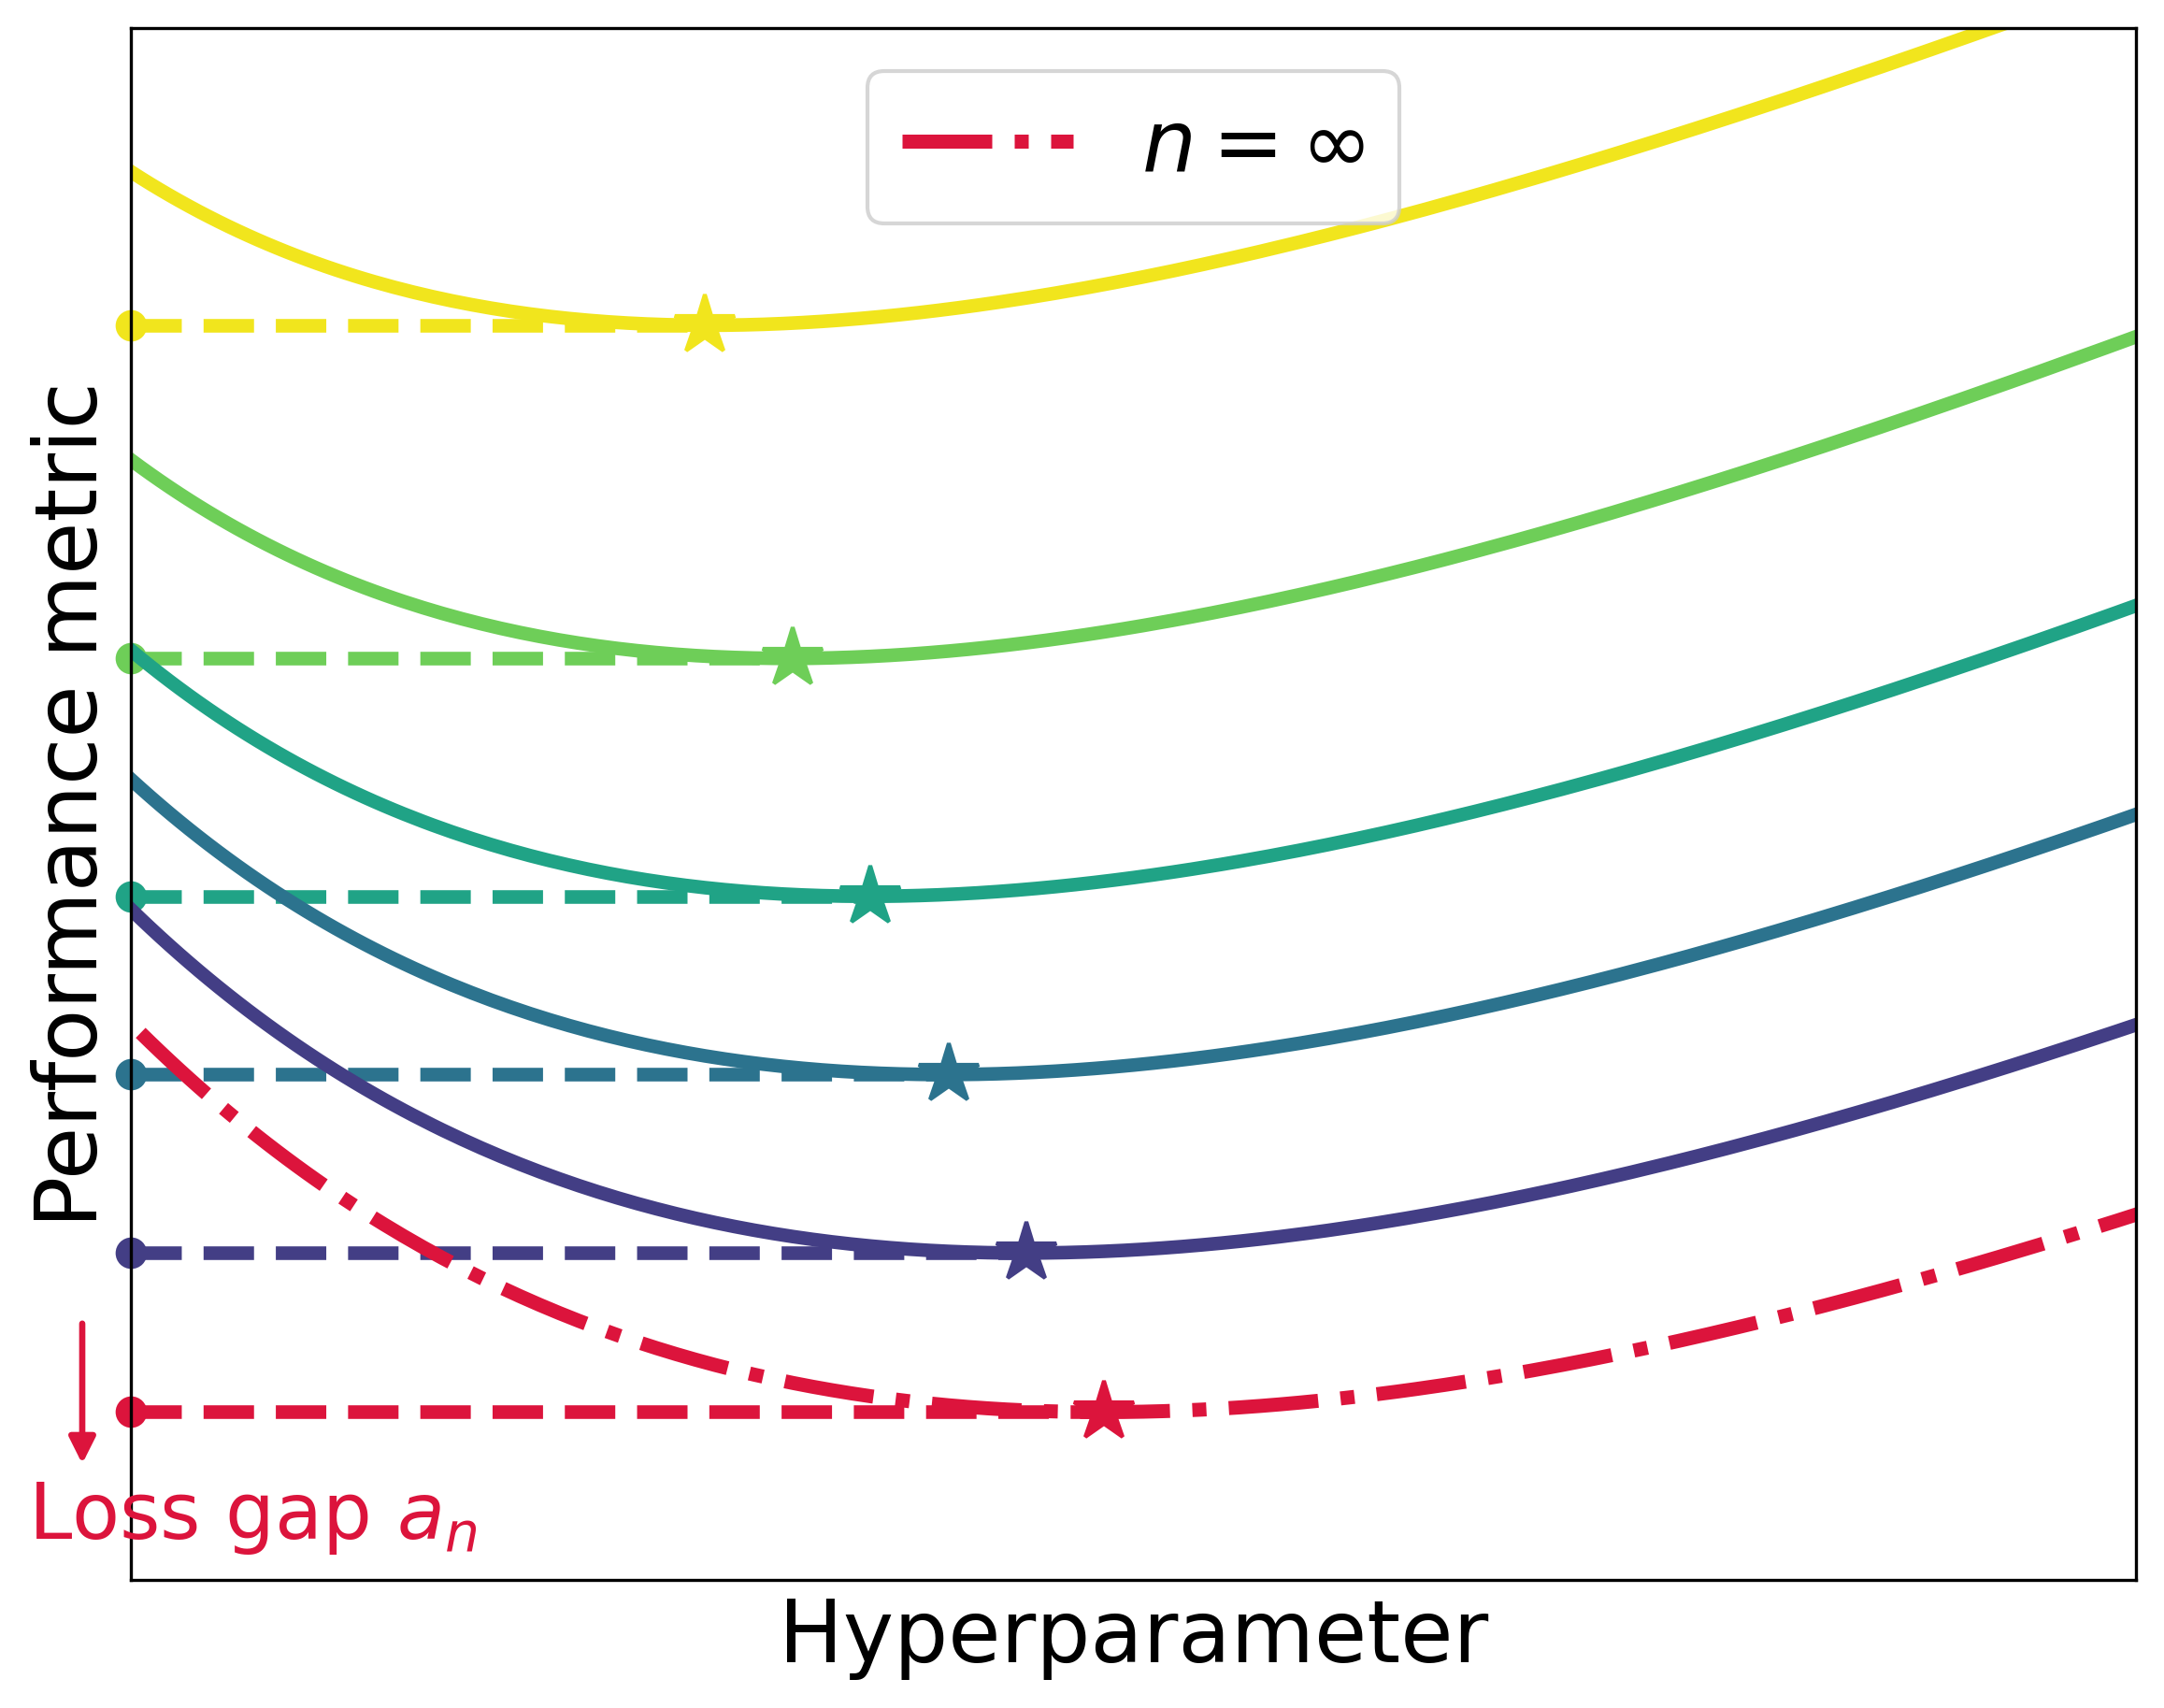
\includegraphics[width=0.98\linewidth]{figure/a_n.png}
    }
    \only<2|handout:0>{%
      \centering
      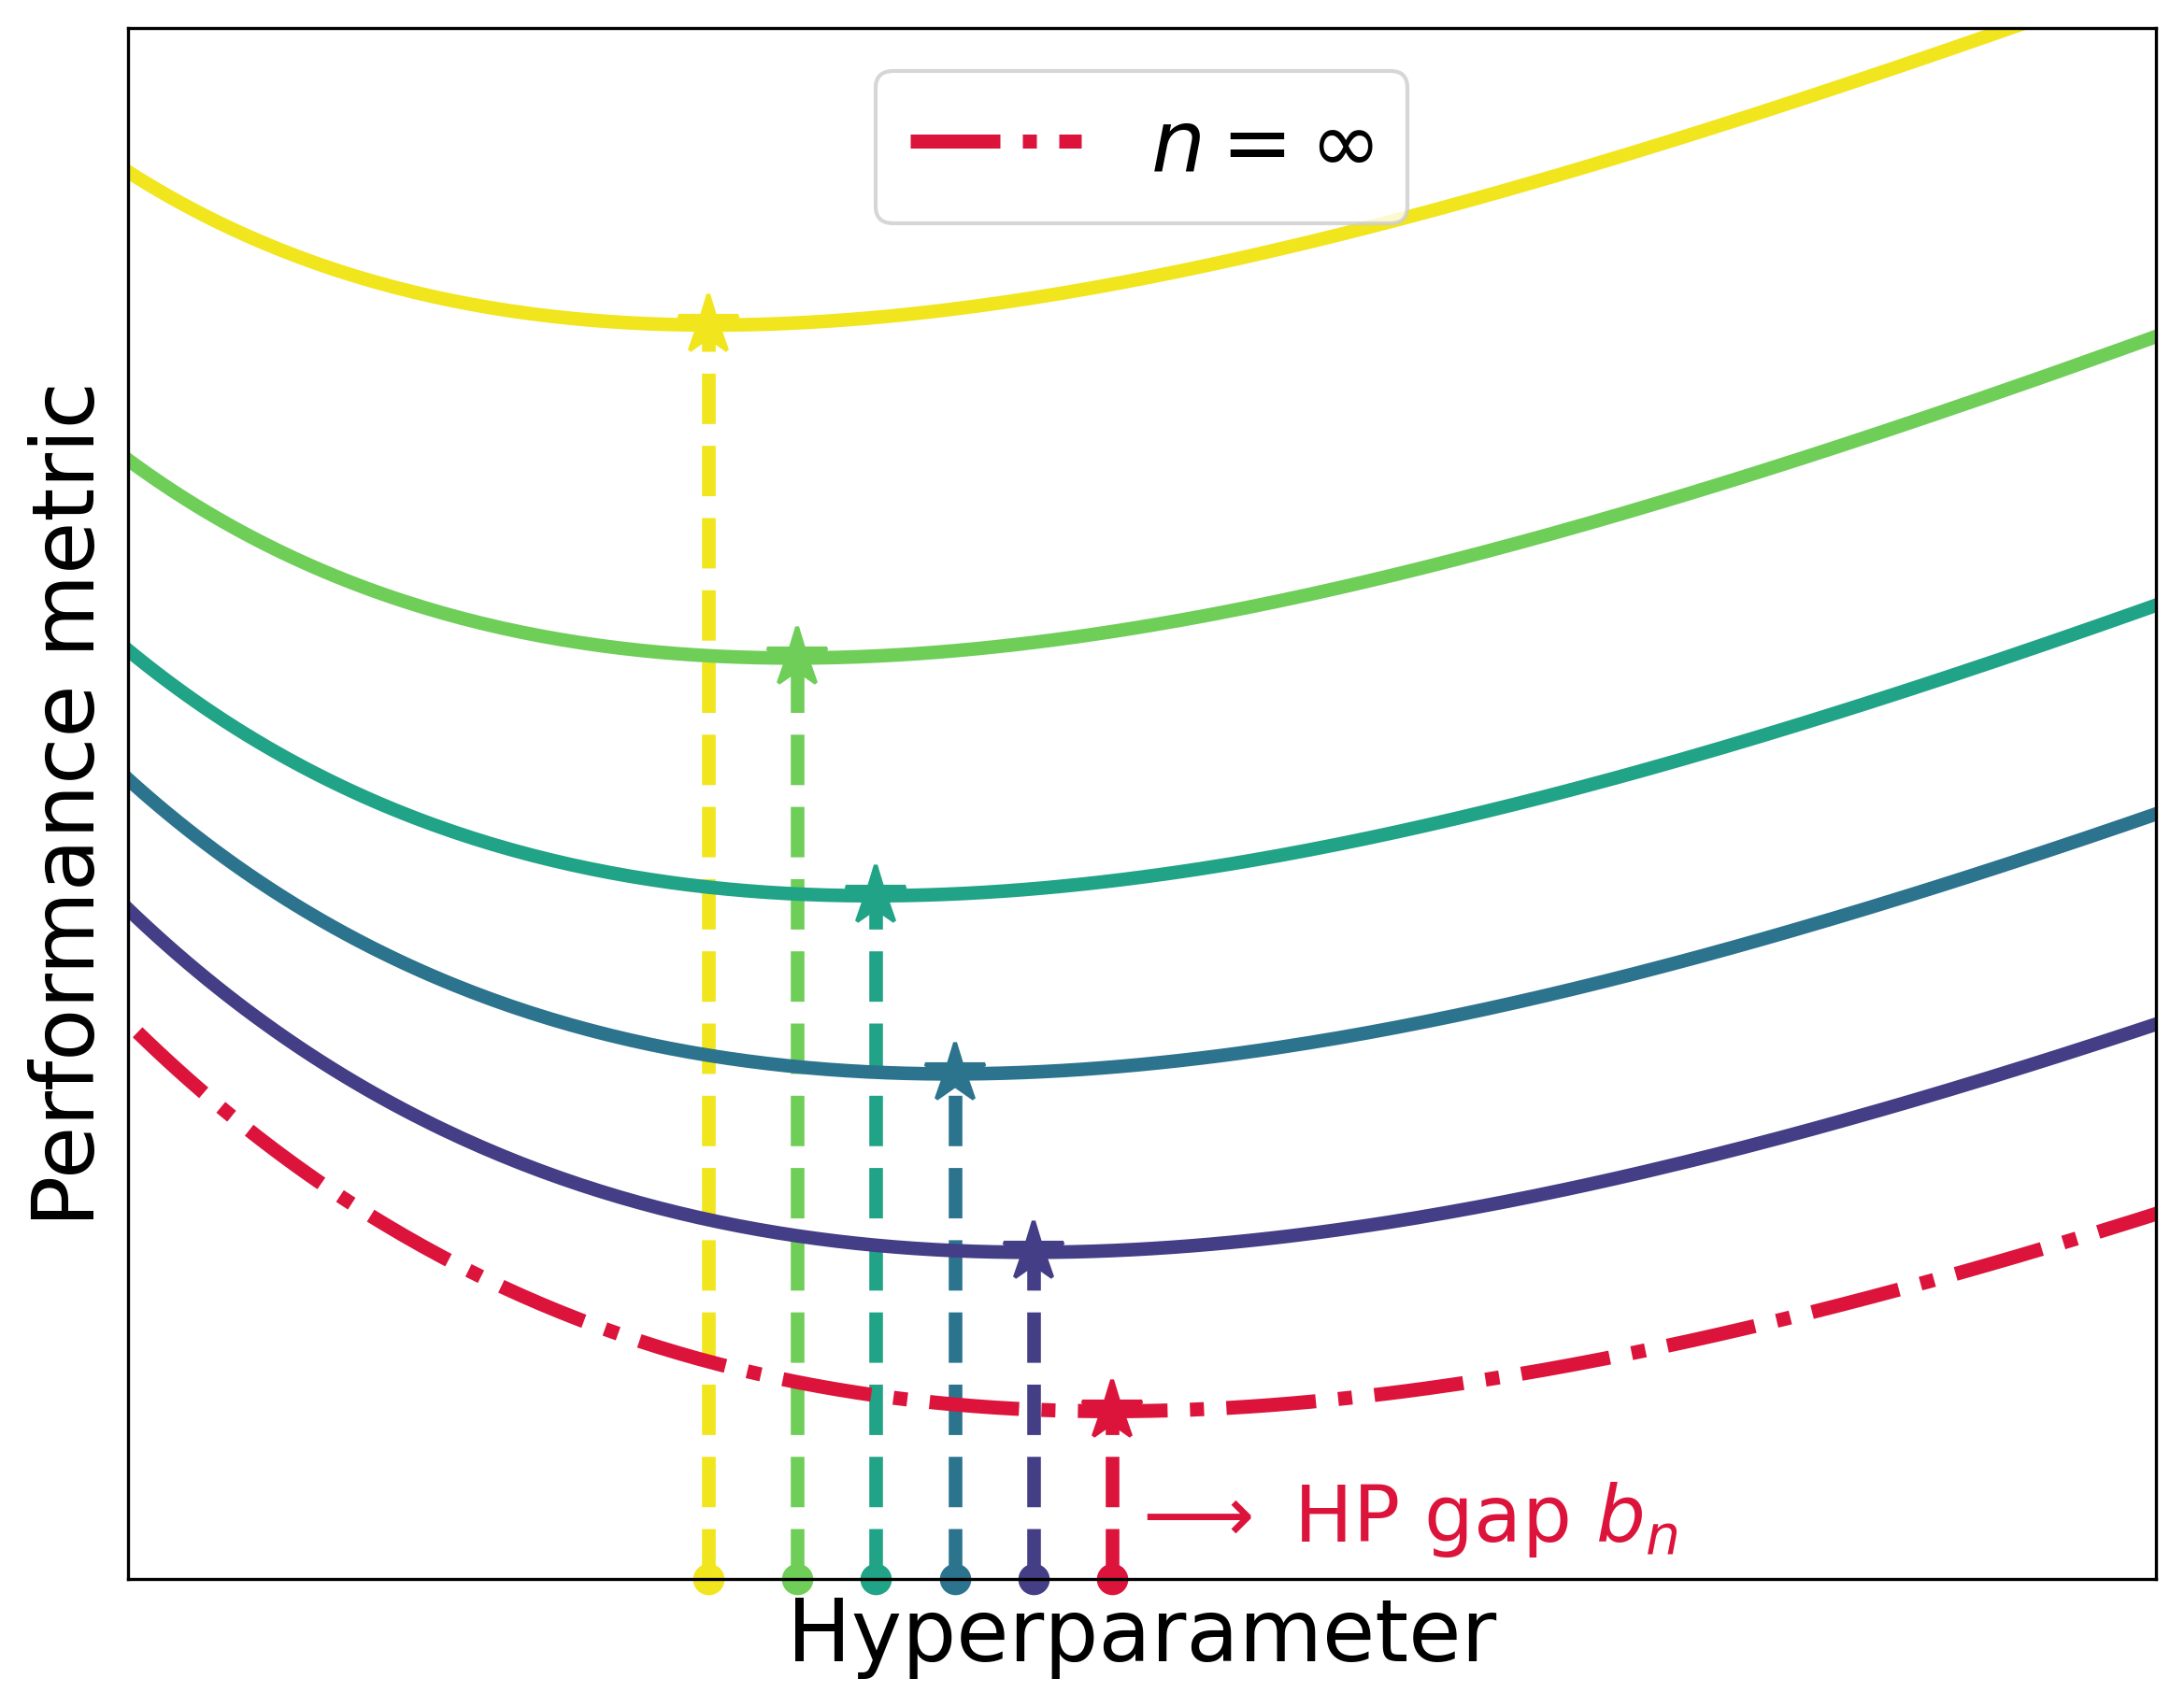
\includegraphics[width=0.98\linewidth]{figure/b_n.png}
    }
    \only<3->{%
      \centering
      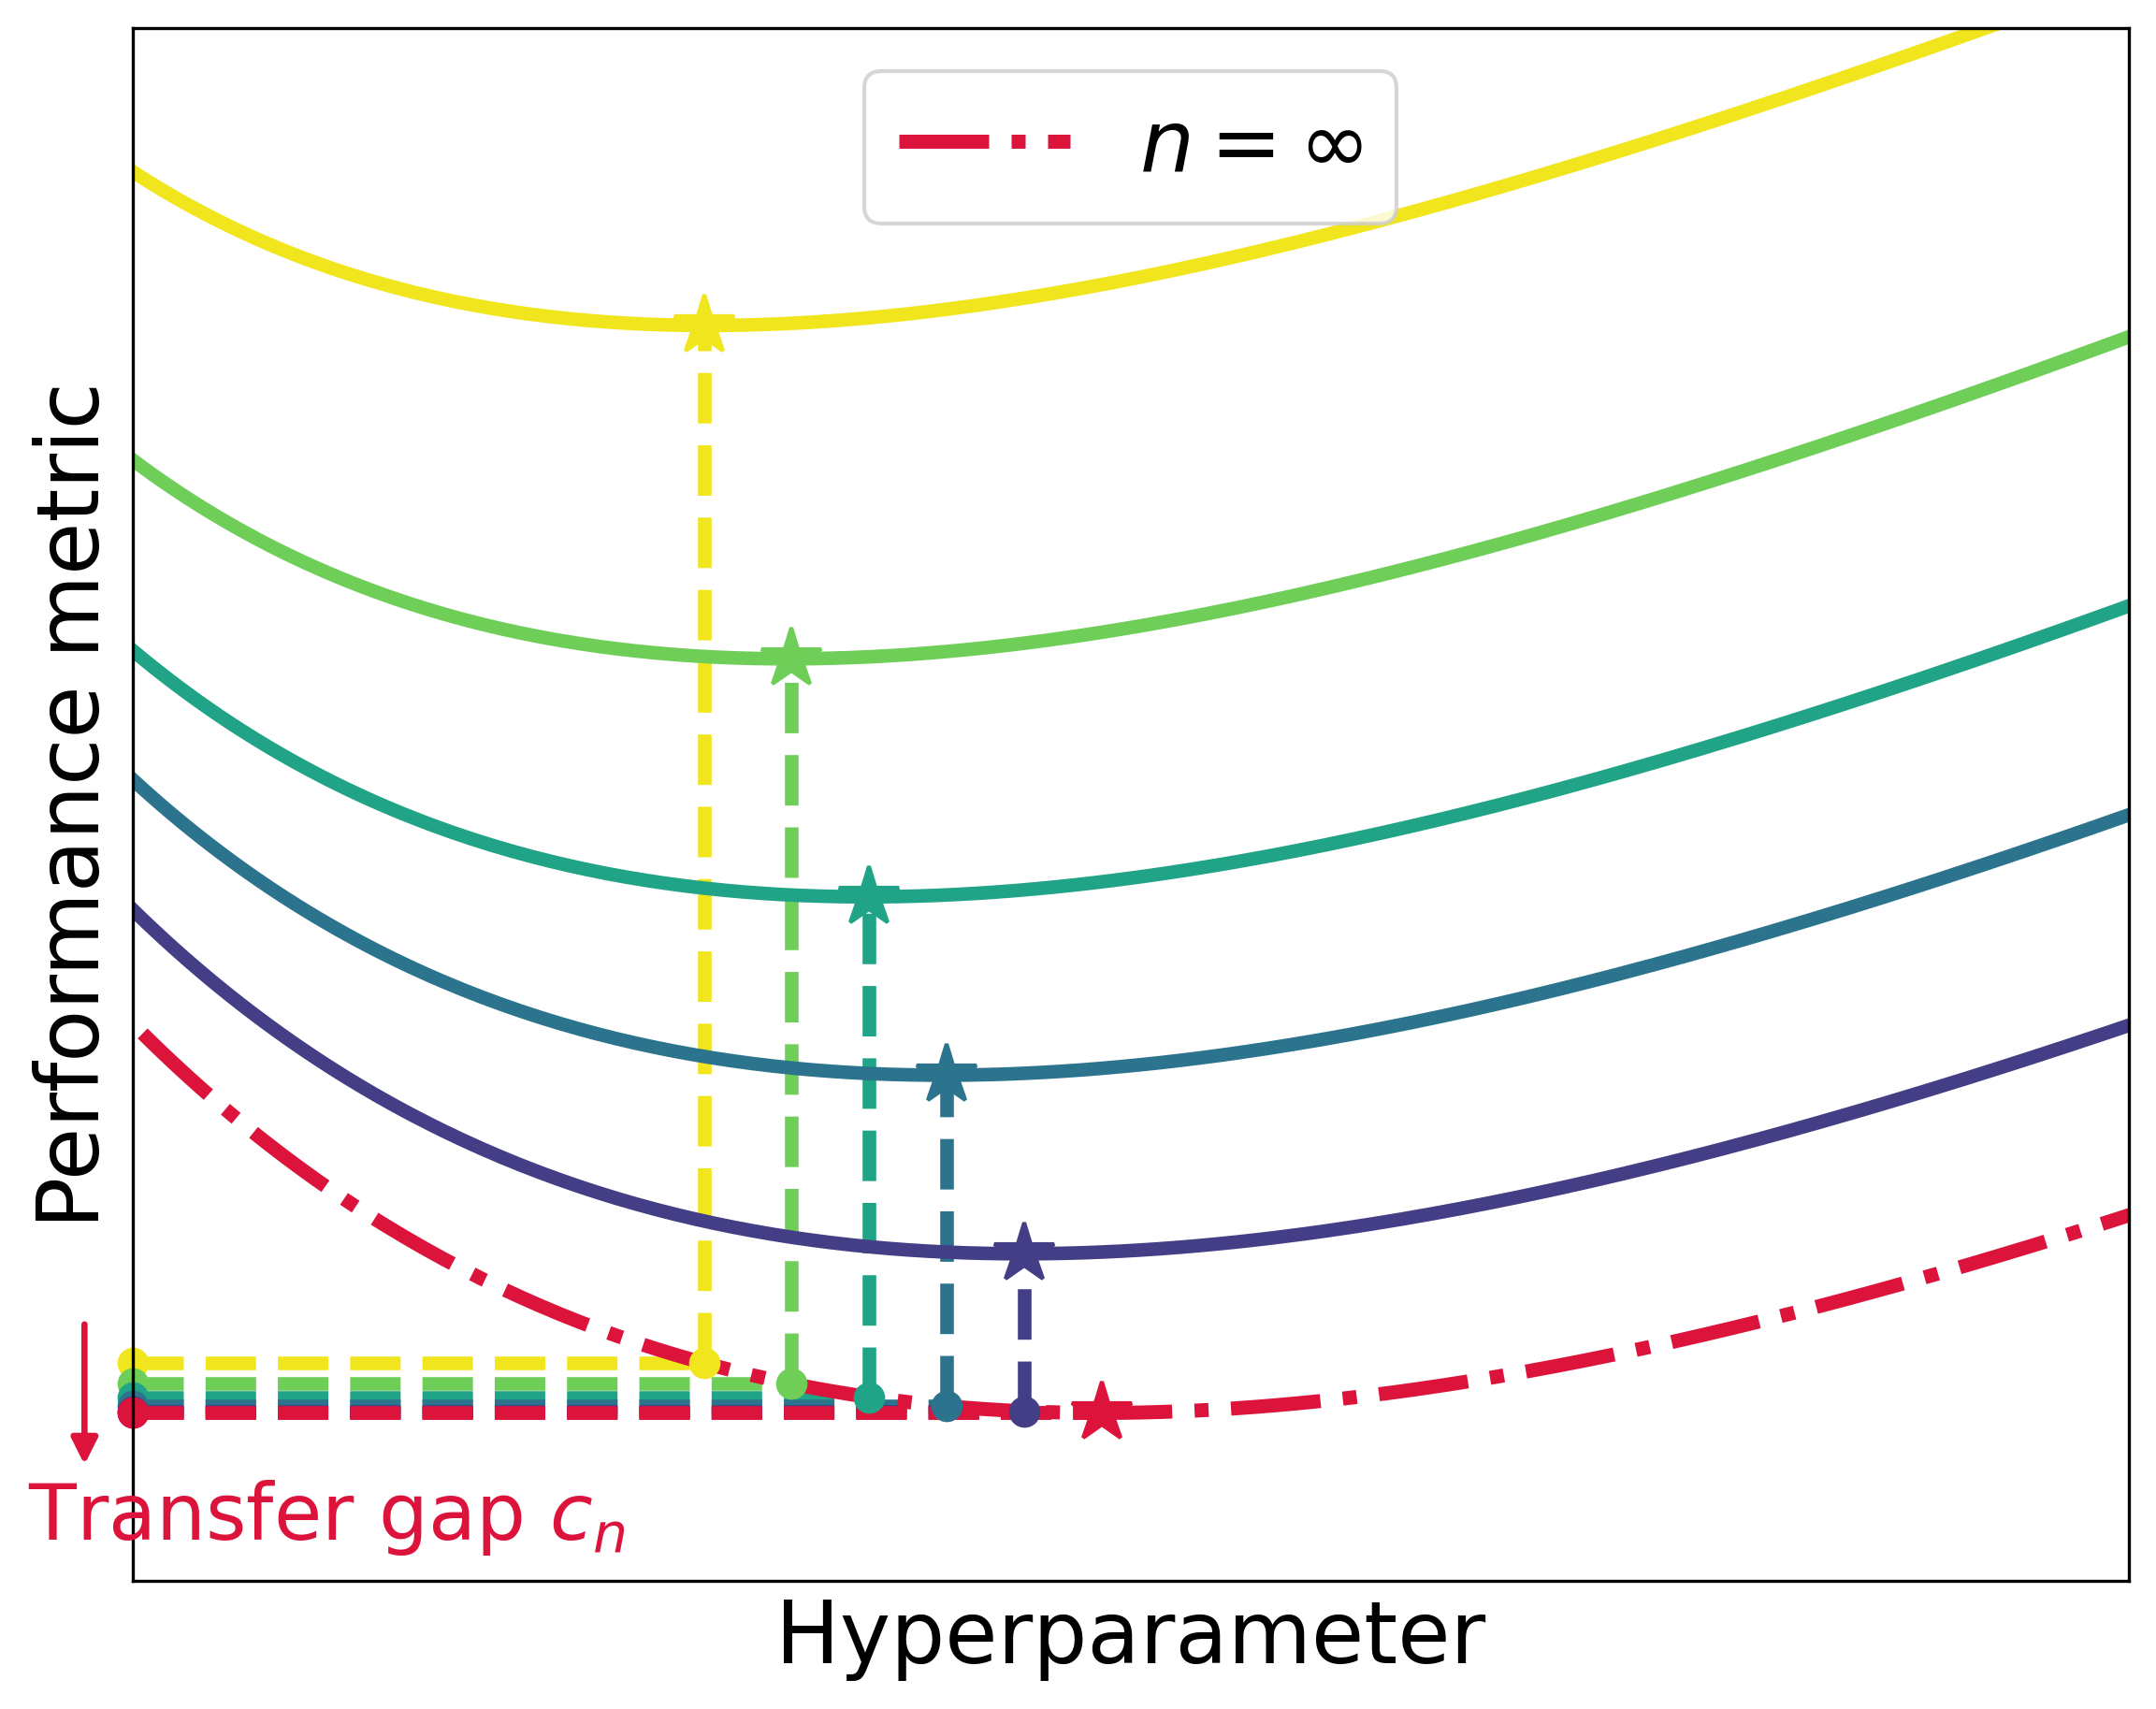
\includegraphics[width=0.98\linewidth]{figure/c_n.png}
    }
  \end{column}
\end{columns}


\end{frame}  

\begin{frame}
\frametitle{A Formal Framework for HP Transfer}
\vspace{1.5mm}

{\small Assume the parameterization gives meaningful HP transfer, i.e., $a_n,b_n,c_n\to 0$. }
\begin{prop}[\small{\color{FlatironOrange2} [GWB25]} Convergence under LSC]
Under \textit{local strong convexity} of $\phi_\infty$ around $\vnu_\infty^*$, i.e., $\phi_\infty''(\vnu_\infty) > 0$, we have
\[
\bullet ~ b_n = O(\sqrt{a_n}), ~\quad~
\bullet ~ c_n = \Theta(b_n^2) = O(a_n).
\]
\end{prop} 
\vspace{-1.5mm}

{\small\color{lightgray!60!black} 
\textbf{Remark:} LSC entails that model performance meaningfully degrades away from the optimum, i.e., HP selection matters in the large-$n$ limit. 
}

\vspace{4mm}

\pause

\hrule

\vspace{2.7mm}

{\small 
Note that under the LSC condition, $c_n$ never converges slower than $a_n$. 
}

\begin{alertblock}{}
We say HP transfer is \textbf{fast} if $c_n = o(a_n)$, i.e., suboptimality gap $c_n$ converges faster than what is naively implied by the \textit{curvature} of $\phi_\infty$. 
\end{alertblock}

\vspace{0.75mm}
\pause

\textbf{Question:} Does this fast transfer definition imply computational gain?


% \begin{prop}[\small{\color{FlatironOrange2} [GWB25]} ``Useful'' Transfer]
% Under \textit{local strong convexity} of $\phi_\infty$ around $\vnu_\infty^*$, we have
% \[
% \bullet ~ b_n = O(\sqrt{a_n}), \quad~
% \bullet ~ c_n = \Theta(b_n^2) = O(a_n).
% \]
% \end{prop} 
\end{frame}  

\begin{frame}
\frametitle{From Fast to Useful Transfer}
\vspace{1.25mm}

{\small
\color{lightgray!60!black} 
Assume $(i)$ total compute budget $\cF$ FLOPS, and $(ii)$ training cost scales as $n^q$. 
% \begin{itemize}\color{lightgray!60!black} 
    % \item Assume $(i)$ total compute budget $\cF$ FLOPS, and $(ii)$ training cost scales as $n^r$.
    % \item Denote $a_n\sim n^{-\alpha}$, $b_n\sim n^{-\beta}$. 
% \end{itemize}

\vspace{2.4mm}
\hrule
\vspace{1.5mm}
}

{

\small

Recall the following strategies of HP sweep. 
\vspace{-1.5mm}
\begin{itemize}\setlength\itemsep{0.2em}
    \item[\ding{112}] \colorbox{teal!12}{\textbf{Direct}}: Grid search on \textit{scale-$n$ model}; compute-optimal performance {$\phi_{\text{dir}}(\cF)$}. 
    % \[
    % \text{$\Rightarrow$~ Compute-optimal performance scales as \colorbox{orange!12}{$\cF^{-\frac{2\alpha}{h\alpha+2r}}$}.} 
    % \]
    \item[\ding{112}] \colorbox{teal!12}{\textbf{Transfer}}: Grid search on \textit{scale-$n$ model}, and transfer to scale-$M$ model ($M\gg n$).\!\!\!\! 
    % \\
    % compute-optimal performance \underline{$\phi_{\text{trans}}(\cF)$}. 
    % \[
    % \text{$\Rightarrow$~ Compute-optimal performance scales as \colorbox{orange!12}{$\cF^{-\frac{\alpha}{r}} + \cF^{-\frac{2\beta}{h\beta+r}}$}.} 
    % \]
\end{itemize}
}


\pause
\vspace{1.5mm}

\begin{alertblock}{}
\centering
We say HP transfer is \textbf{useful} if $\abs{\phi_{\text{trans}}(\cF) - \phi_\infty^*} \ll \abs{\phi_{\text{dir}}(\cF) - \phi_\infty^*}$. 
\end{alertblock}
\vspace{-2.5mm}

{\small
\color{lightgray!60!black} i.e., under the same compute budget, transfer yields lower loss than direct tuning. 
}

\pause
\vspace{1.5mm}

\vspace{2.5mm}
\hrule
\vspace{1.5mm}

{\small
\color{lightgray!60!black} 
The definitions and fast and useful transfer coincides under the LSC condition.
}

\begin{prop}[\small{\color{FlatironOrange2} [GWB25]} Fast Transfer = Useful Transfer]
Under LSC of $\phi_\infty$, transfer is useful if and only if $c_n {\,\color{lightgray!66!black} = \Theta(b_n^2)} = o(a_n)$. 
\end{prop} 
\vspace{-1mm}

\pause

{
\begin{itemize}\setlength\itemsep{0.1em}
    \item \textbf{Observation:} under LSC, transfer \underline{\textit{never underperforms}} the direct strategy. 
    % \item \textbf{Question:} when does transfer \textit{\color{FlatironOrange2!90!black}\underline{outperform}} direct tuning?
\end{itemize}

}

\end{frame}  

\begin{frame}
\frametitle{Recap: Definitions and Convergence Rates}
\vspace{1.5mm}

\begin{figure}[t]
\centering
\begin{minipage}[t]{0.32\linewidth}
\centering
{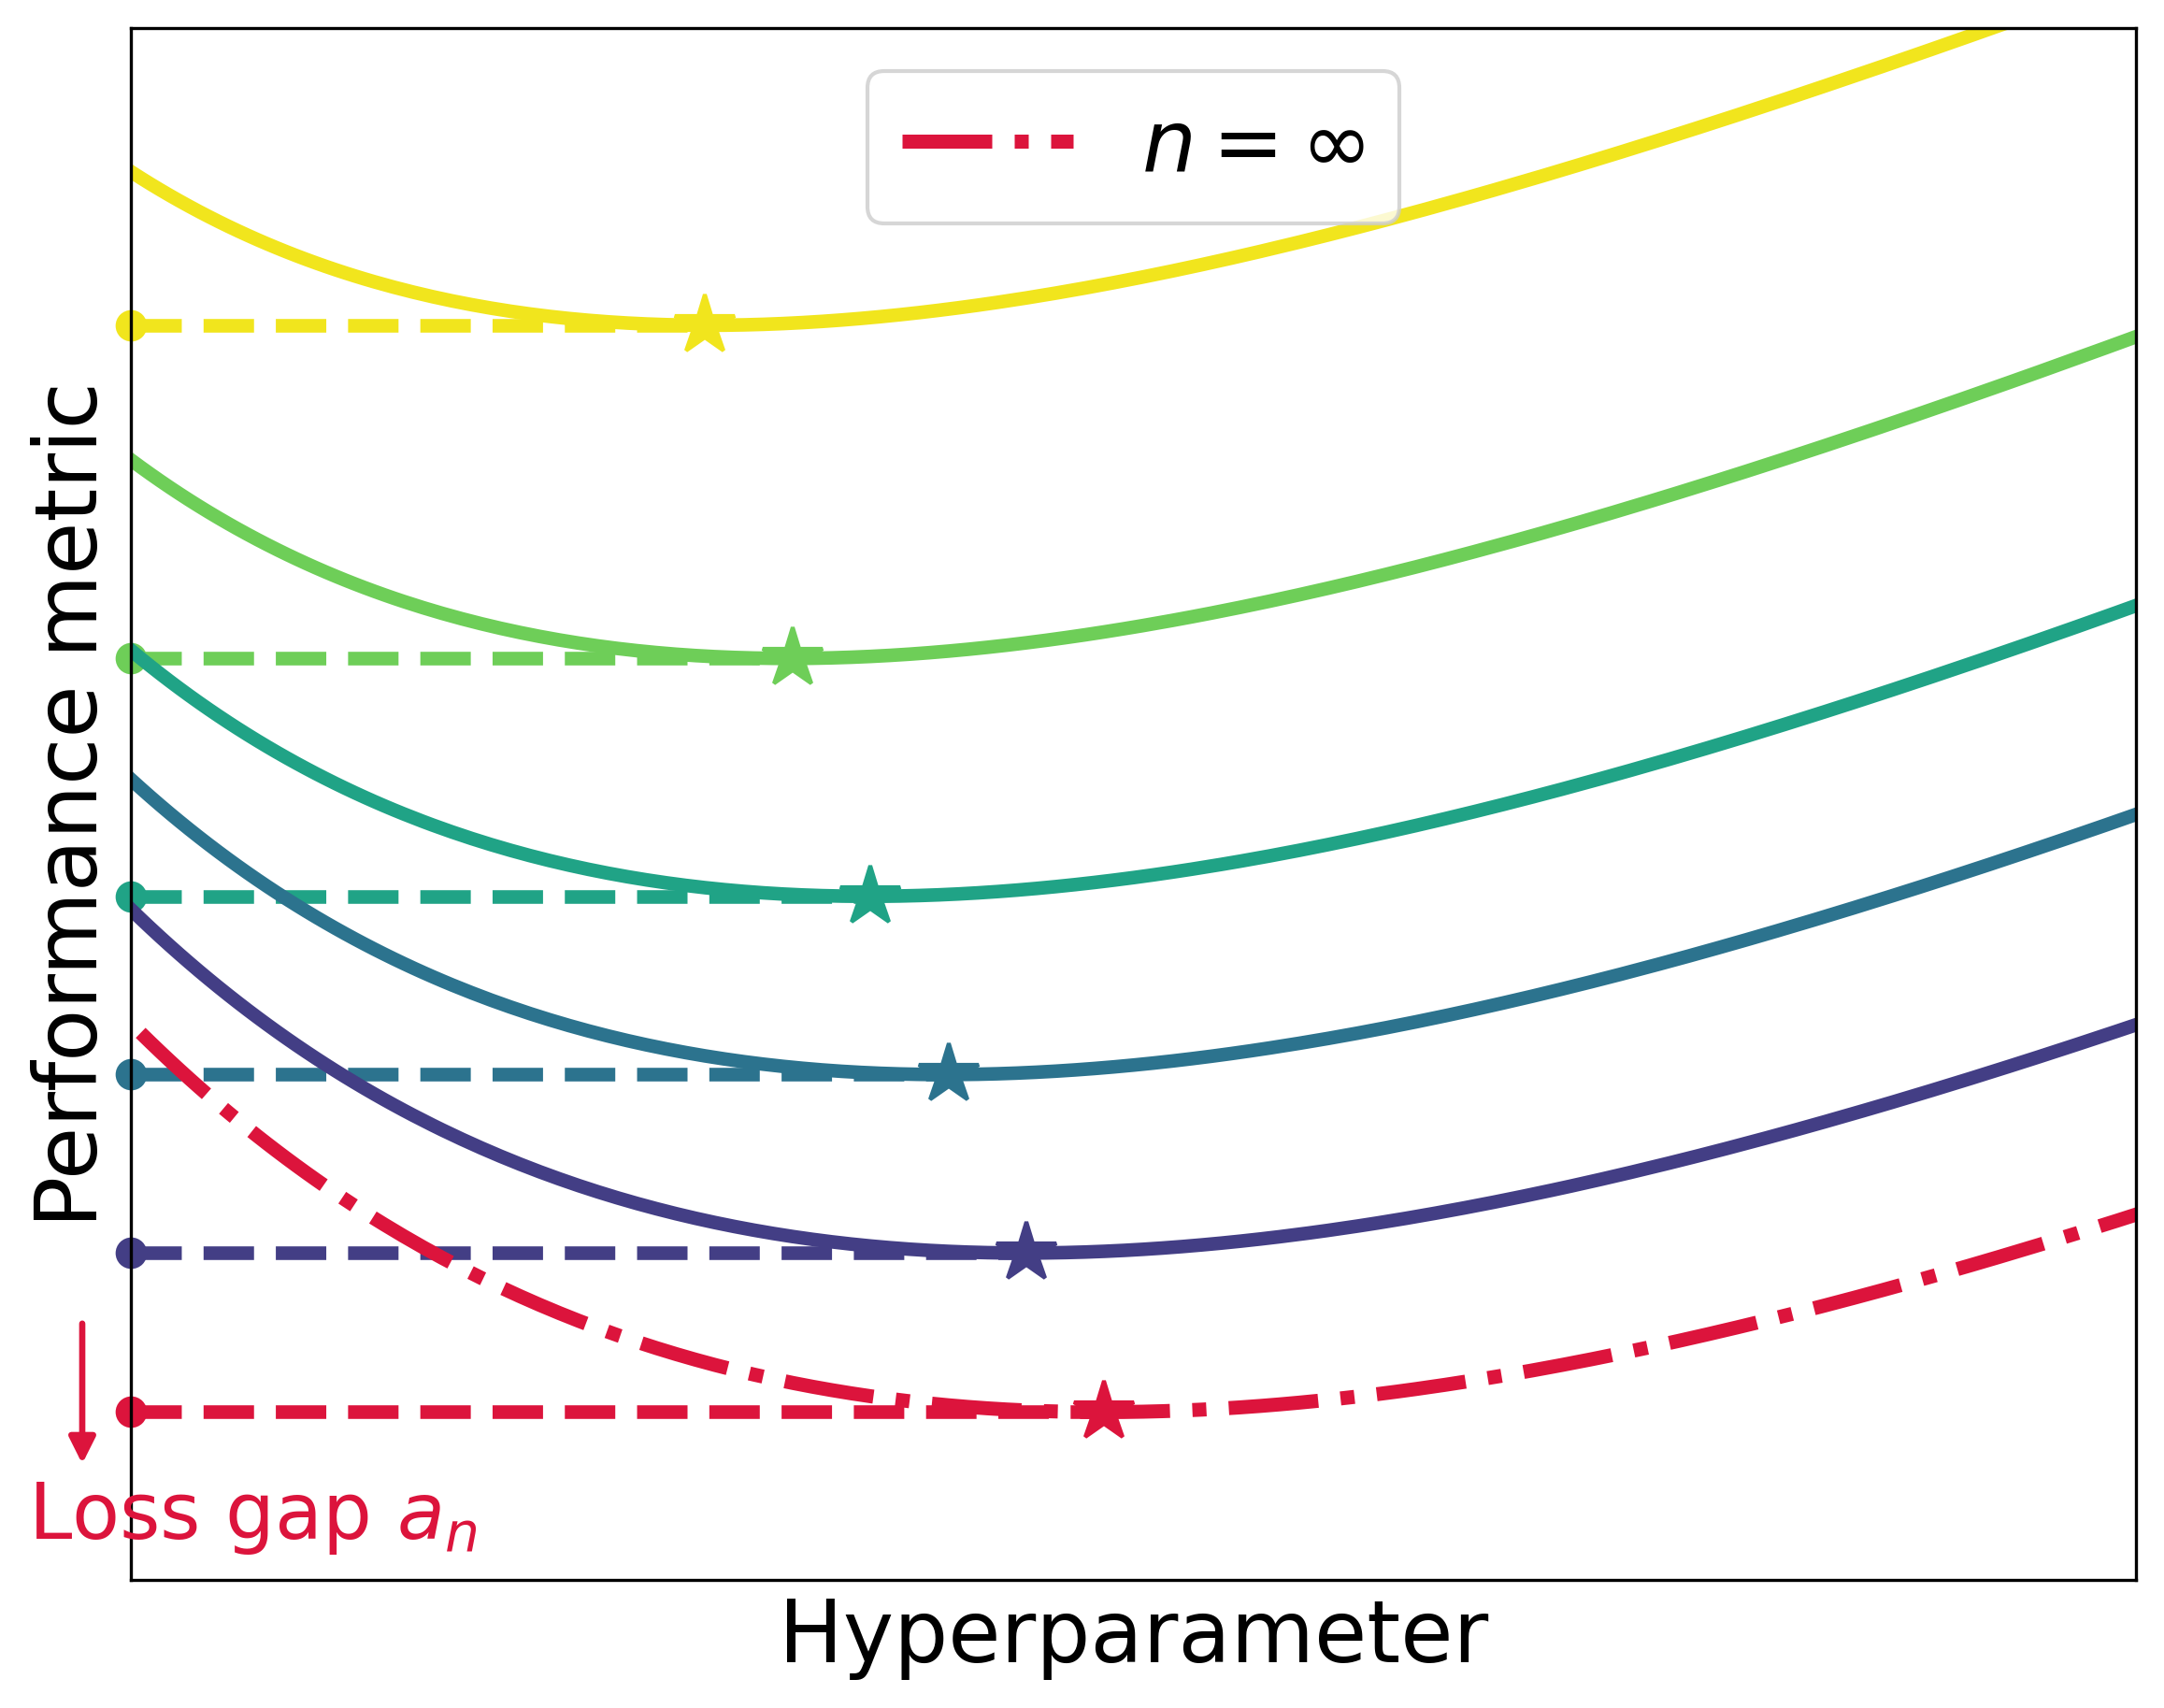
\includegraphics[height=0.75\textwidth]{figure/a_n.png}} \vspace{-2mm}\\
{\small loss gap $a_n$.}
\end{minipage}%
\begin{minipage}[t]{0.32\linewidth}
\centering
{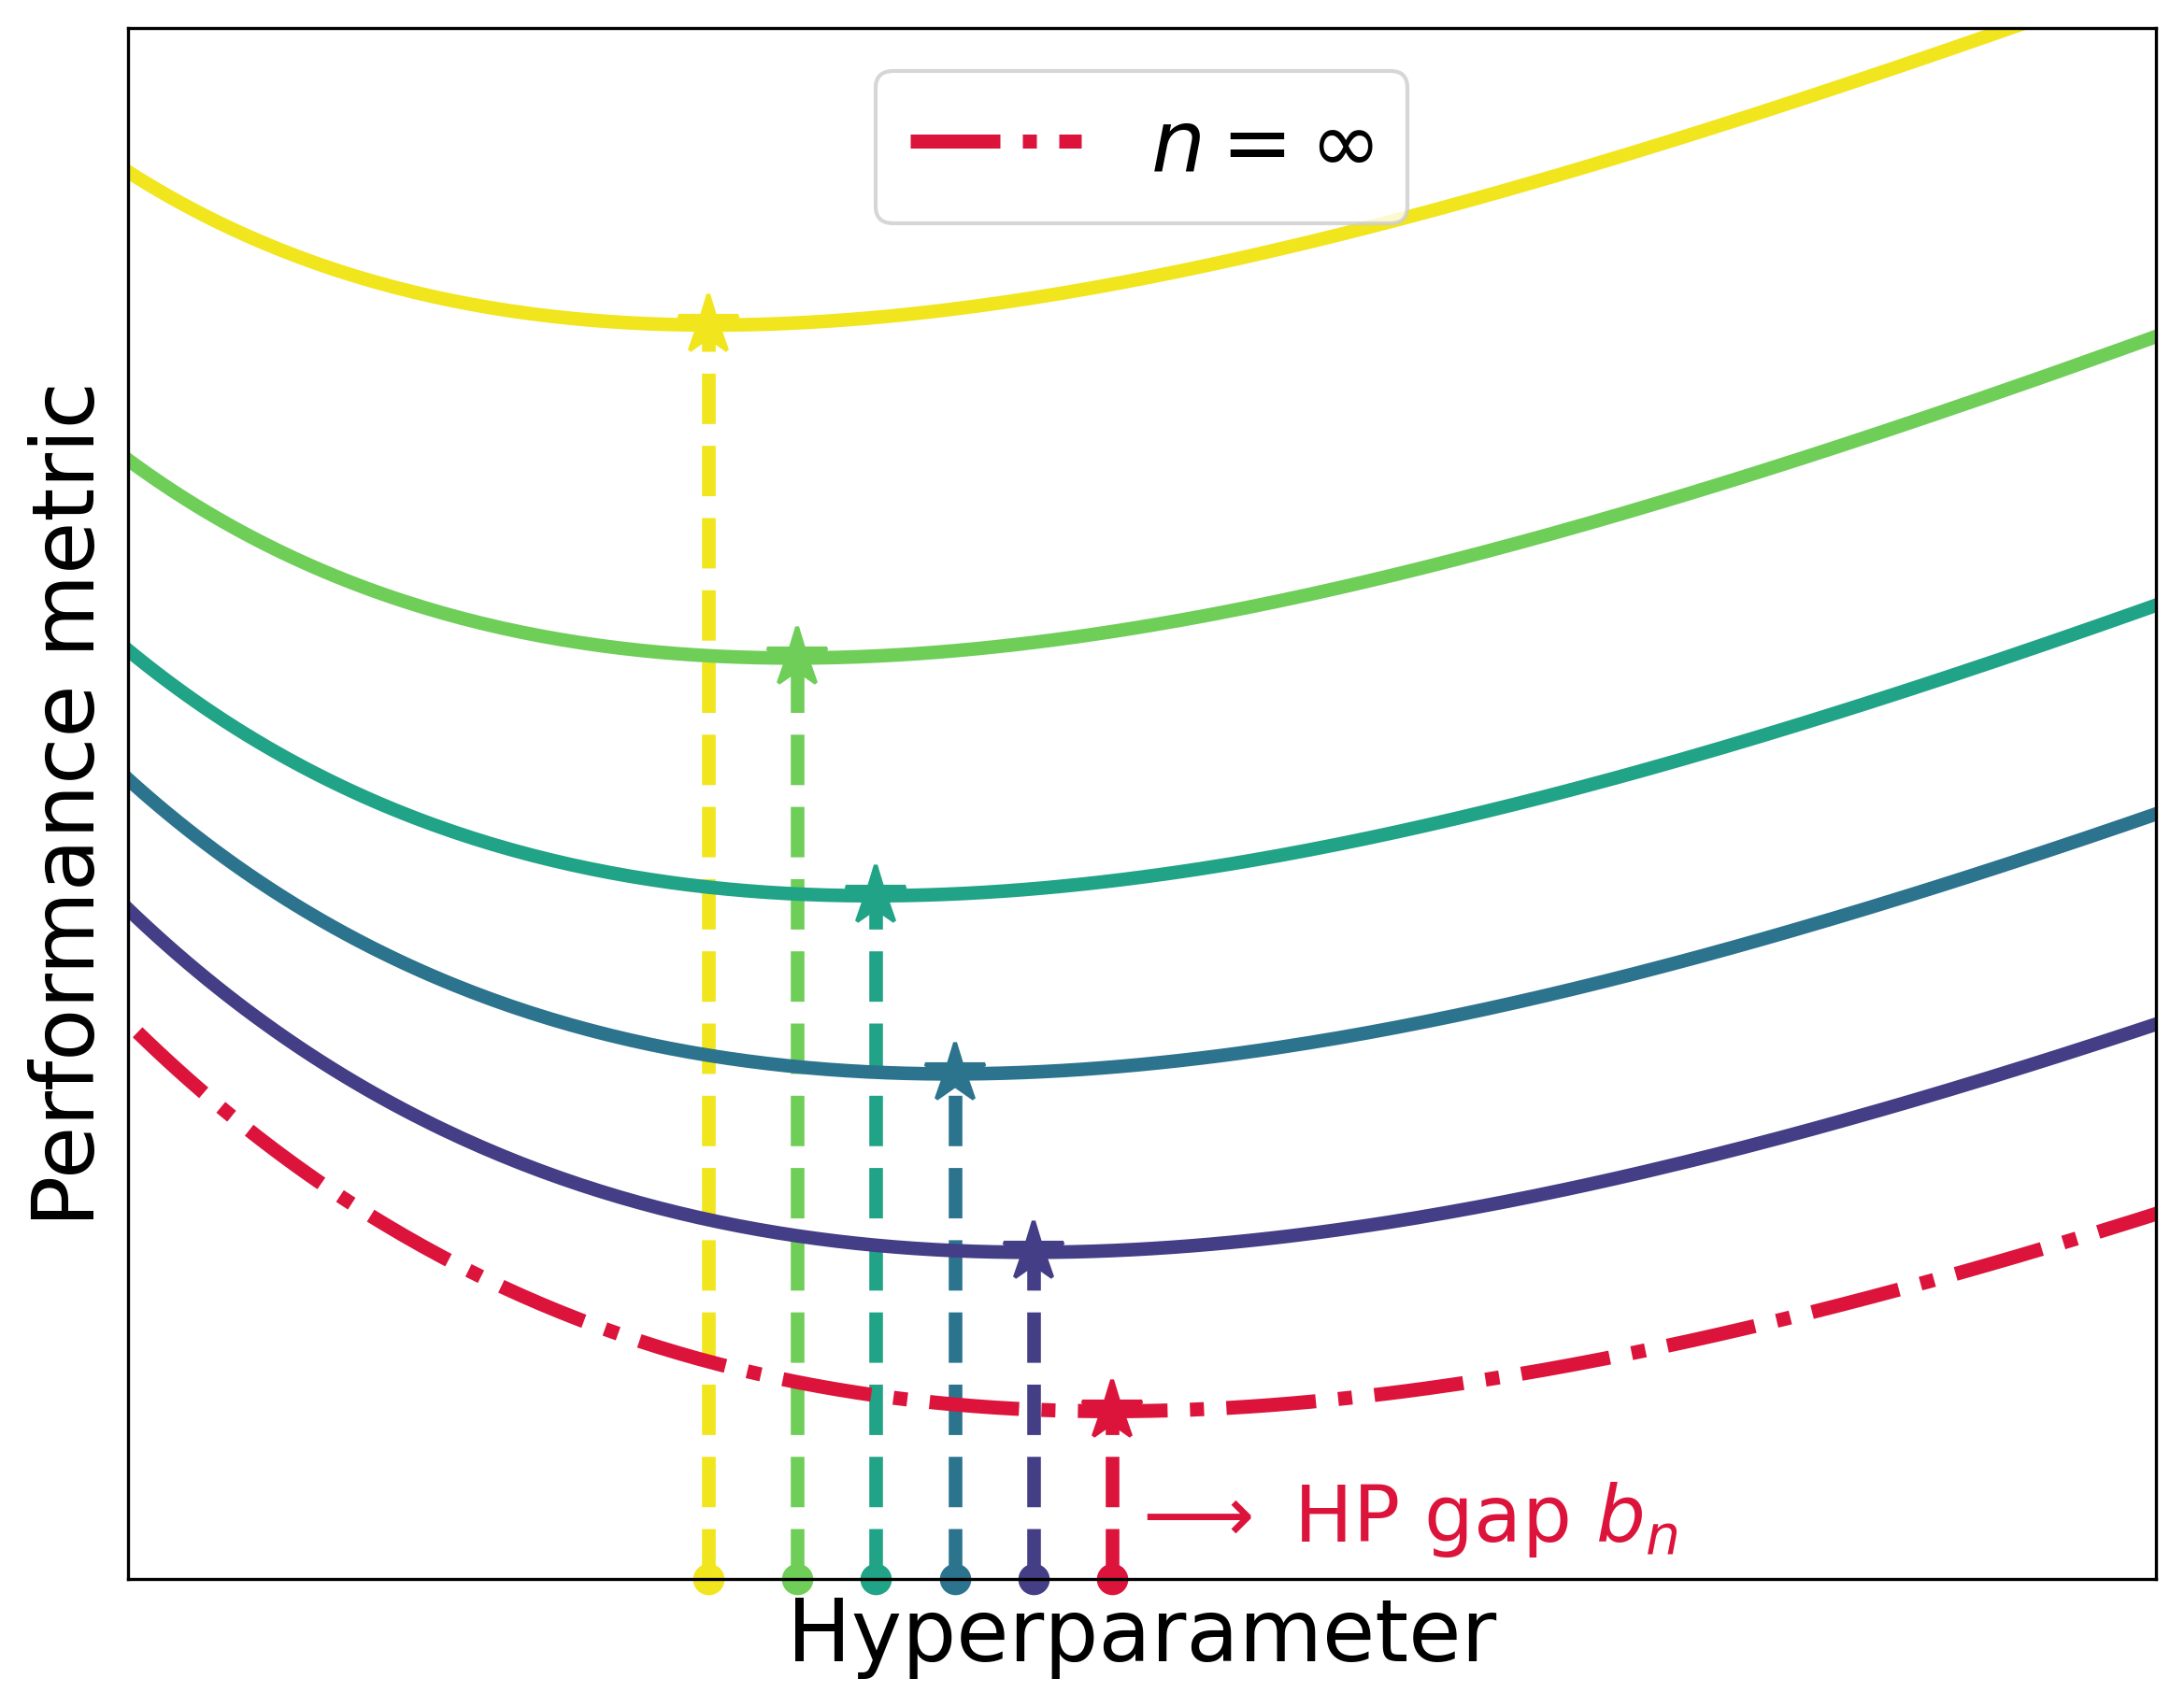
\includegraphics[height=0.75\textwidth]{figure/b_n.png}} \vspace{-2mm}\\
{\small HP gap $b_n$.} 
\end{minipage}
\begin{minipage}[t]{0.32\linewidth}
\centering
{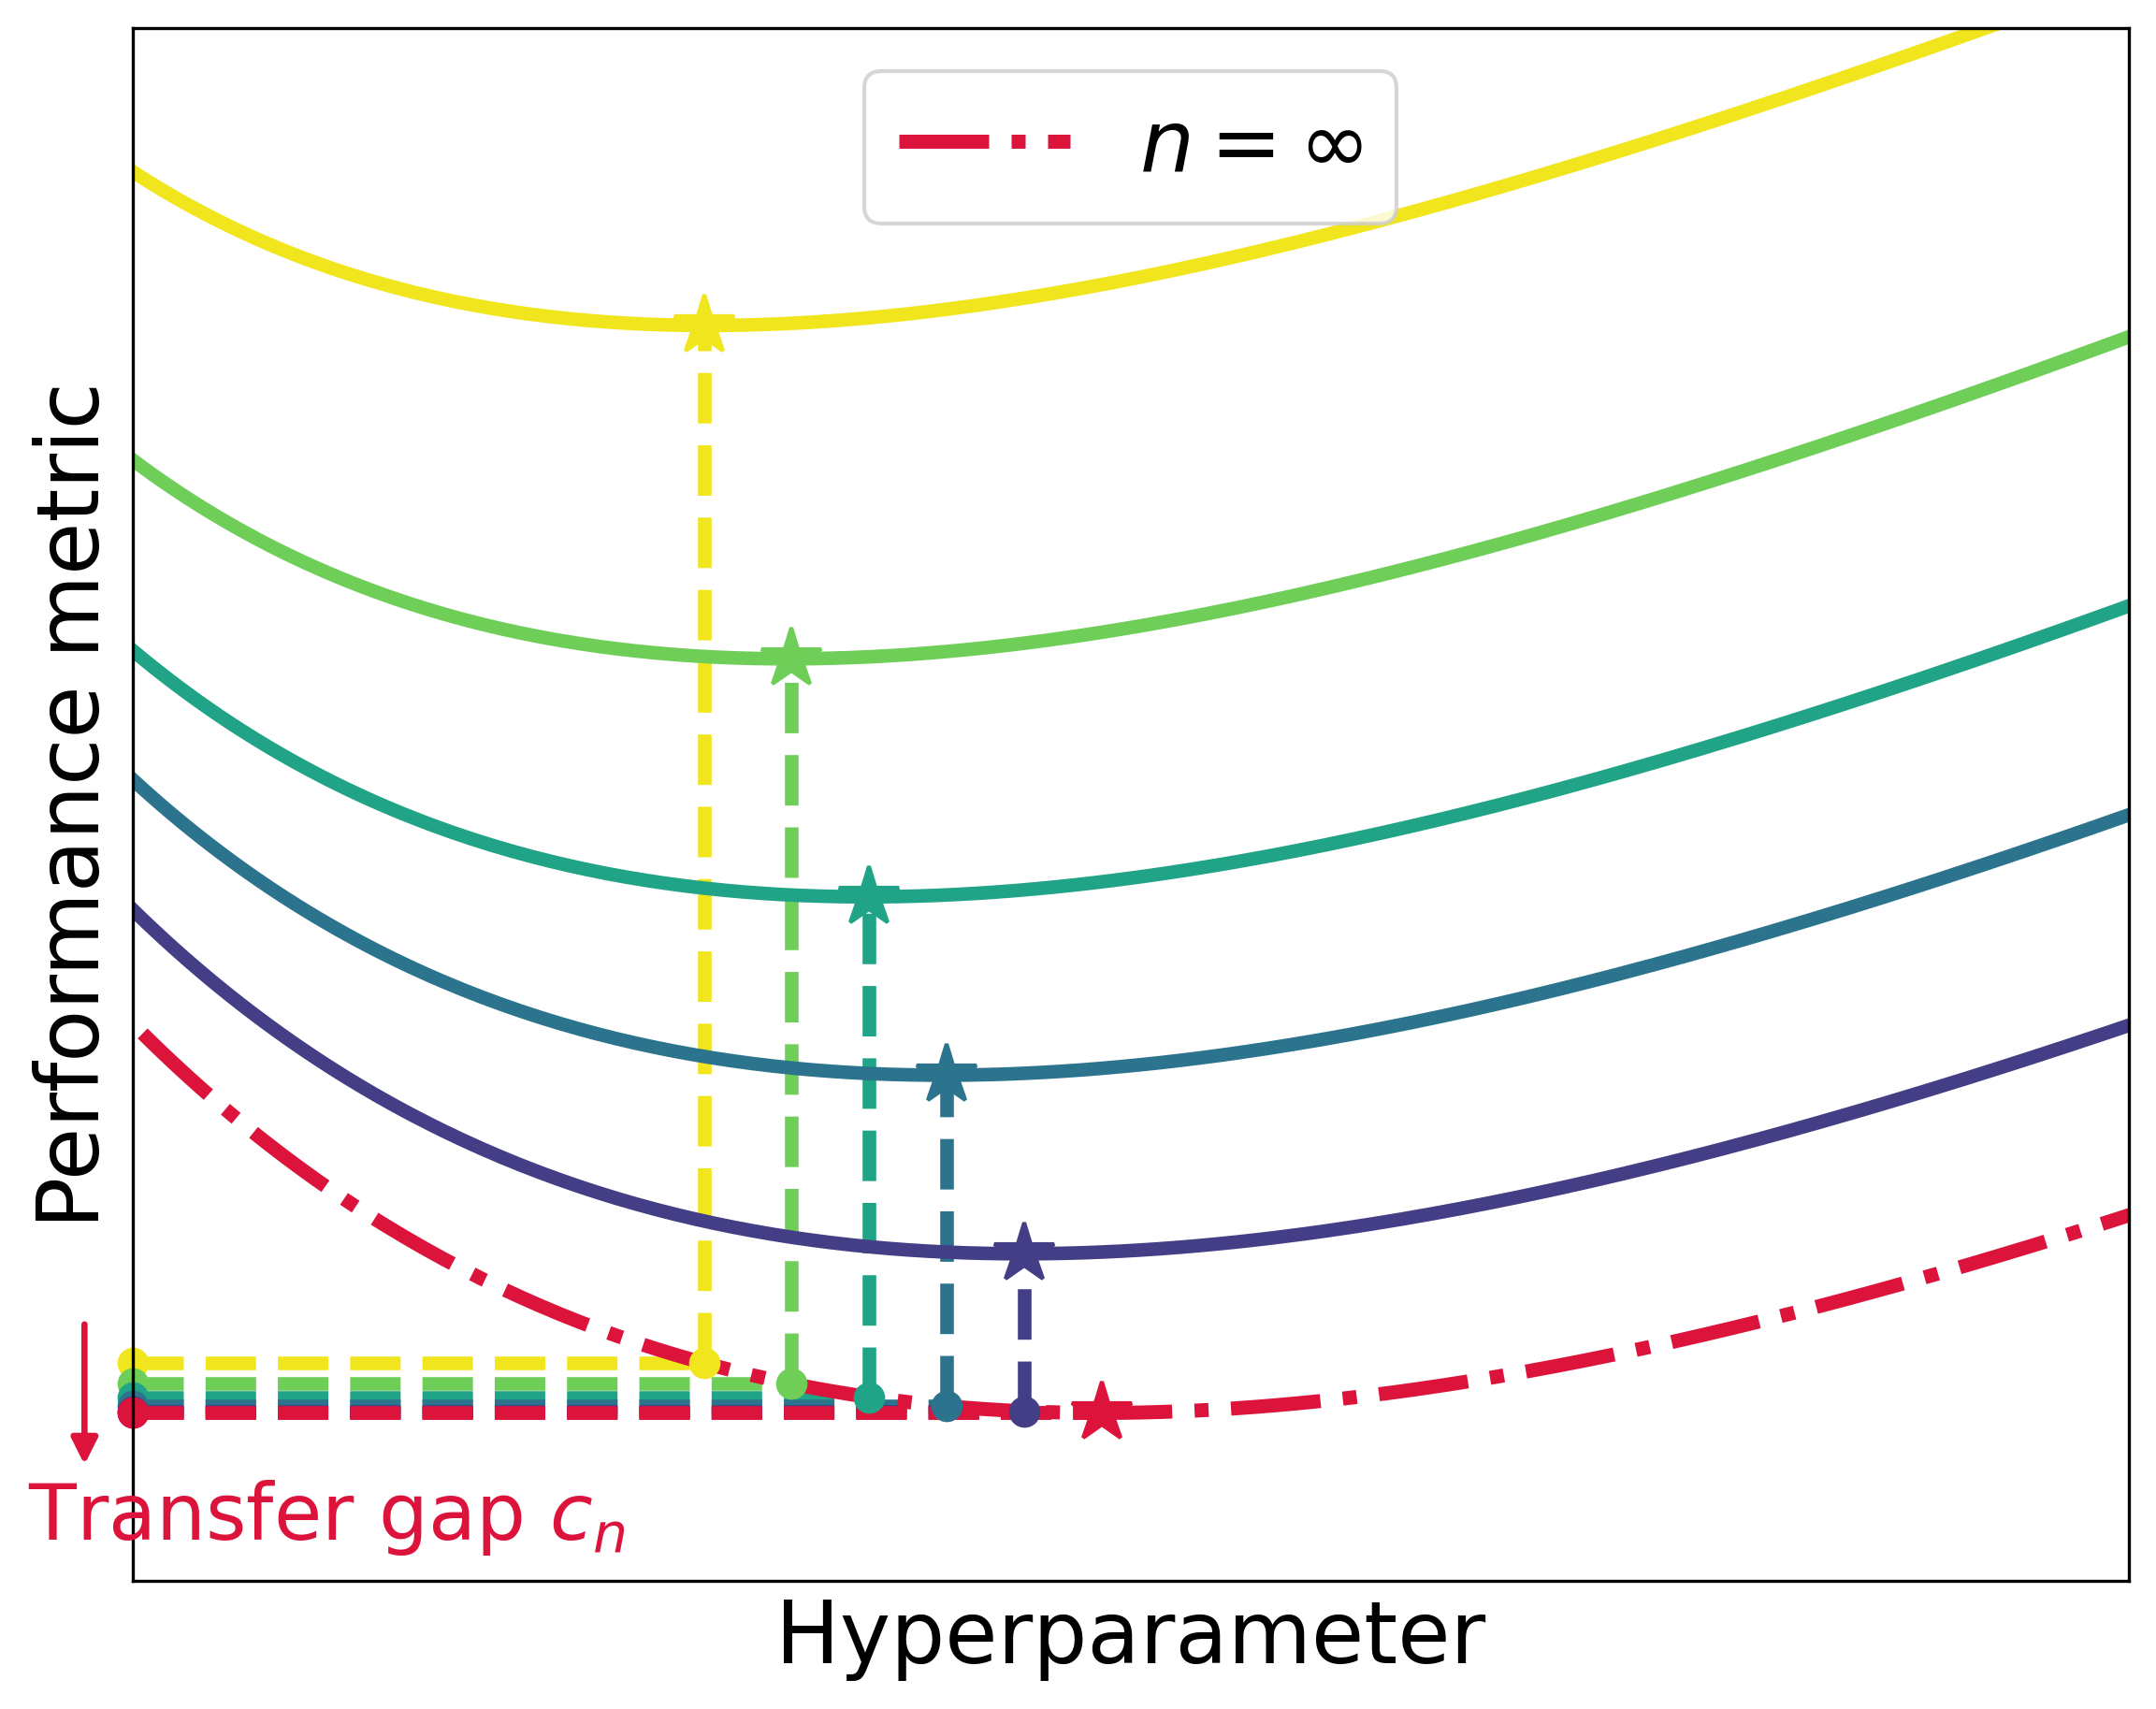
\includegraphics[height=0.75\textwidth]{figure/c_n.png}} \vspace{-2mm}\\
{\small transfer gap $c_n$.} 
\end{minipage}
% \vspace{-5mm}
% \vspace{-2mm}
\end{figure}


\begin{block}{}
\begin{itemize}
    \item[\ding{112}] \textbf{Agnostic rate:} \textit{local strong convexity} of $\phi_\infty$ implies \colorbox{red!12}{$c_n = O(a_n)$}. 
    \item[\ding{112}] \textbf{Usefulness:} transfer provides computational gain iff \colorbox{blue!12}{$c_n = o(a_n)$}.
\end{itemize}
\end{block}

\pause

{
\vspace{4.2mm}
\hrule
\vspace{2mm}


\textbf{Question:} when does transfer \textit{\color{FlatironOrange2!90!black}\underline{outperform}} direct tuning, i.e., $c_n\ll a_n$? 

\small 
\begin{itemize}\color{lightgray!60!black} 
    \item[$\frownie$] Scaling exponents in $a_n,b_n,c_n$ difficult to quantify, except for \textit{synthetic settings}. 
\end{itemize}


}



\end{frame}  

\begin{frame}
\frametitle{Example of Fast Transfer}
\vspace{1.5mm}

{\small
\begin{itemize}\setlength\itemsep{0.42em} 
    \item \textbf{\colorbox{teal!12}{Task}: Gaussian Single-index Model.} 
    {\color{lightgray!60!black} $y = \sigma_*(\langle\vx,\vbeta_*\rangle) + \varepsilon, \quad \text{where~ } \vx\sim\mathcal{N}(0,\vI_d), ~ \norm{\vbeta_*}=1, ~\mathrm{Var}(\varepsilon) = \sigma_\varepsilon^2.$}
    \item \textbf{\colorbox{teal!12}{Model}: Random Features Ridge Estimator.} 
    {\color{lightgray!60!black} $f(\vx) = \langle\va_\lambda, \sigma(\vW\vx)\rangle, 
    \quad \text{where~ } \vW\in\R^{d\times n}, ~
    [\vW]_{i,j}\sim \mathcal{N}(0,1/d)$,  
    $\textstyle\va_\lambda := \mathrm{argmin}_{\va\in\R^n} \sum_{i=1}^N (y_i - \langle\va, \sigma(\vW\vx_i)\rangle)^2 + \lambda\norm{\va}_2^2.$}
    \item \textbf{\colorbox{teal!12}{Regime}: Proportional Limit.} $N,d,n\to\infty;\, N/d\to\psi_1, n/d\to\psi_2\in (0,\infty)$. \\
    {\color{lightgray!60!black} Increasing scale $\,\Rightarrow\,$ larger model width $\psi_2 = n/d$. }
\end{itemize}
}

\vspace{2.5mm}
\pause

\begin{prop}[\small{\color{FlatironOrange2} [GWB25]} Fast Transfer of $\ell_2$ Regularization]

Define $\lambda^*_{\psi_2} := \argmin_{\lambda\in\R} \cR_{\psi_2}(\lambda)$, where $\cR_{\psi_2}(\lambda)$ is the prediction risk, then
\begin{itemize}\setlength\itemsep{0.36em} 
    \item[\ding{112}] \textbf{Loss gap {\color{FlatironOrange2!90!black}$a_n$}:} $|{\cR_{\psi_2}(\lambda^*_{\psi_2}) - \cR_{\infty}(\lambda^*_{\infty})}| = \Theta({\color{blue}\psi_2^{-1})}$. 
    \item[\ding{112}] \textbf{Hyperparameter gap {\color{FlatironOrange2!90!black}$b_n$}:} $|{\lambda^*_{\psi_2} - \lambda^*_{\infty})}| = O({\color{blue}\psi_2^{-1}})$.  \pause
    \item[\ding{112}] \textbf{Suboptimality gap {\color{FlatironOrange2!90!black}$c_n$}:} $|{\cR_\infty(\lambda^*_{\psi_2}) - \cR_\infty(\lambda^*_{\infty}))}| = O({\color{red!80!black}\psi_2^{-2}})$. 
\end{itemize}

\end{prop} 


\end{frame}  

\begin{frame}
\frametitle{Example of Fast Transfer}
\vspace{1.6mm} 

\begin{prop}[\small{\color{FlatironOrange2} [GWB25]} Fast Transfer of $\ell_2$ Regularization]

% Define $\lambda^*_{\psi_2} := \argmin_{\lambda\in\R} \cR_{\psi_2}(\lambda)$, where $\cR_{\psi_2}(\lambda)$ is the prediction risk, then
\begin{itemize}\setlength\itemsep{0.36em} 
    \item[\ding{112}] \textbf{Loss gap {\color{FlatironOrange2!90!black}$a_n$}:} $|{\cR_{\psi_2}(\lambda^*_{\psi_2}) - \cR_{\infty}(\lambda^*_{\infty})}| = \Theta({\color{blue}\psi_2^{-1})}$. 
    \item[\ding{112}] \textbf{Hyperparameter gap {\color{FlatironOrange2!90!black}$b_n$}:} $|{\lambda^*_{\psi_2} - \lambda^*_{\infty})}| = O({\color{blue}\psi_2^{-1}})$. 
    \item[\ding{112}] \textbf{Suboptimality gap {\color{FlatironOrange2!90!black}$c_n$}:} $|{\cR_\infty(\lambda^*_{\psi_2}) - \cR_\infty(\lambda^*_{\infty}))}| = O({\color{red!80!black}\psi_2^{-2}})$. 
\end{itemize}

\end{prop} 

\vspace{-1.8mm}

{\small \color{lightgray!60!black} \textbf{Message.} $c_n\ll a_n$: transfer offers computationally gain in tuning $\ell_2$ penalty.}

\begin{figure}[t]
\vspace{-1mm}
\centering
\begin{minipage}[t]{0.49\linewidth}
\centering
{
\includegraphics[height=0.72\textwidth]{figure/RFF_loss.png}}  
\end{minipage}%
\begin{minipage}[t]{0.49\linewidth}
\centering 
{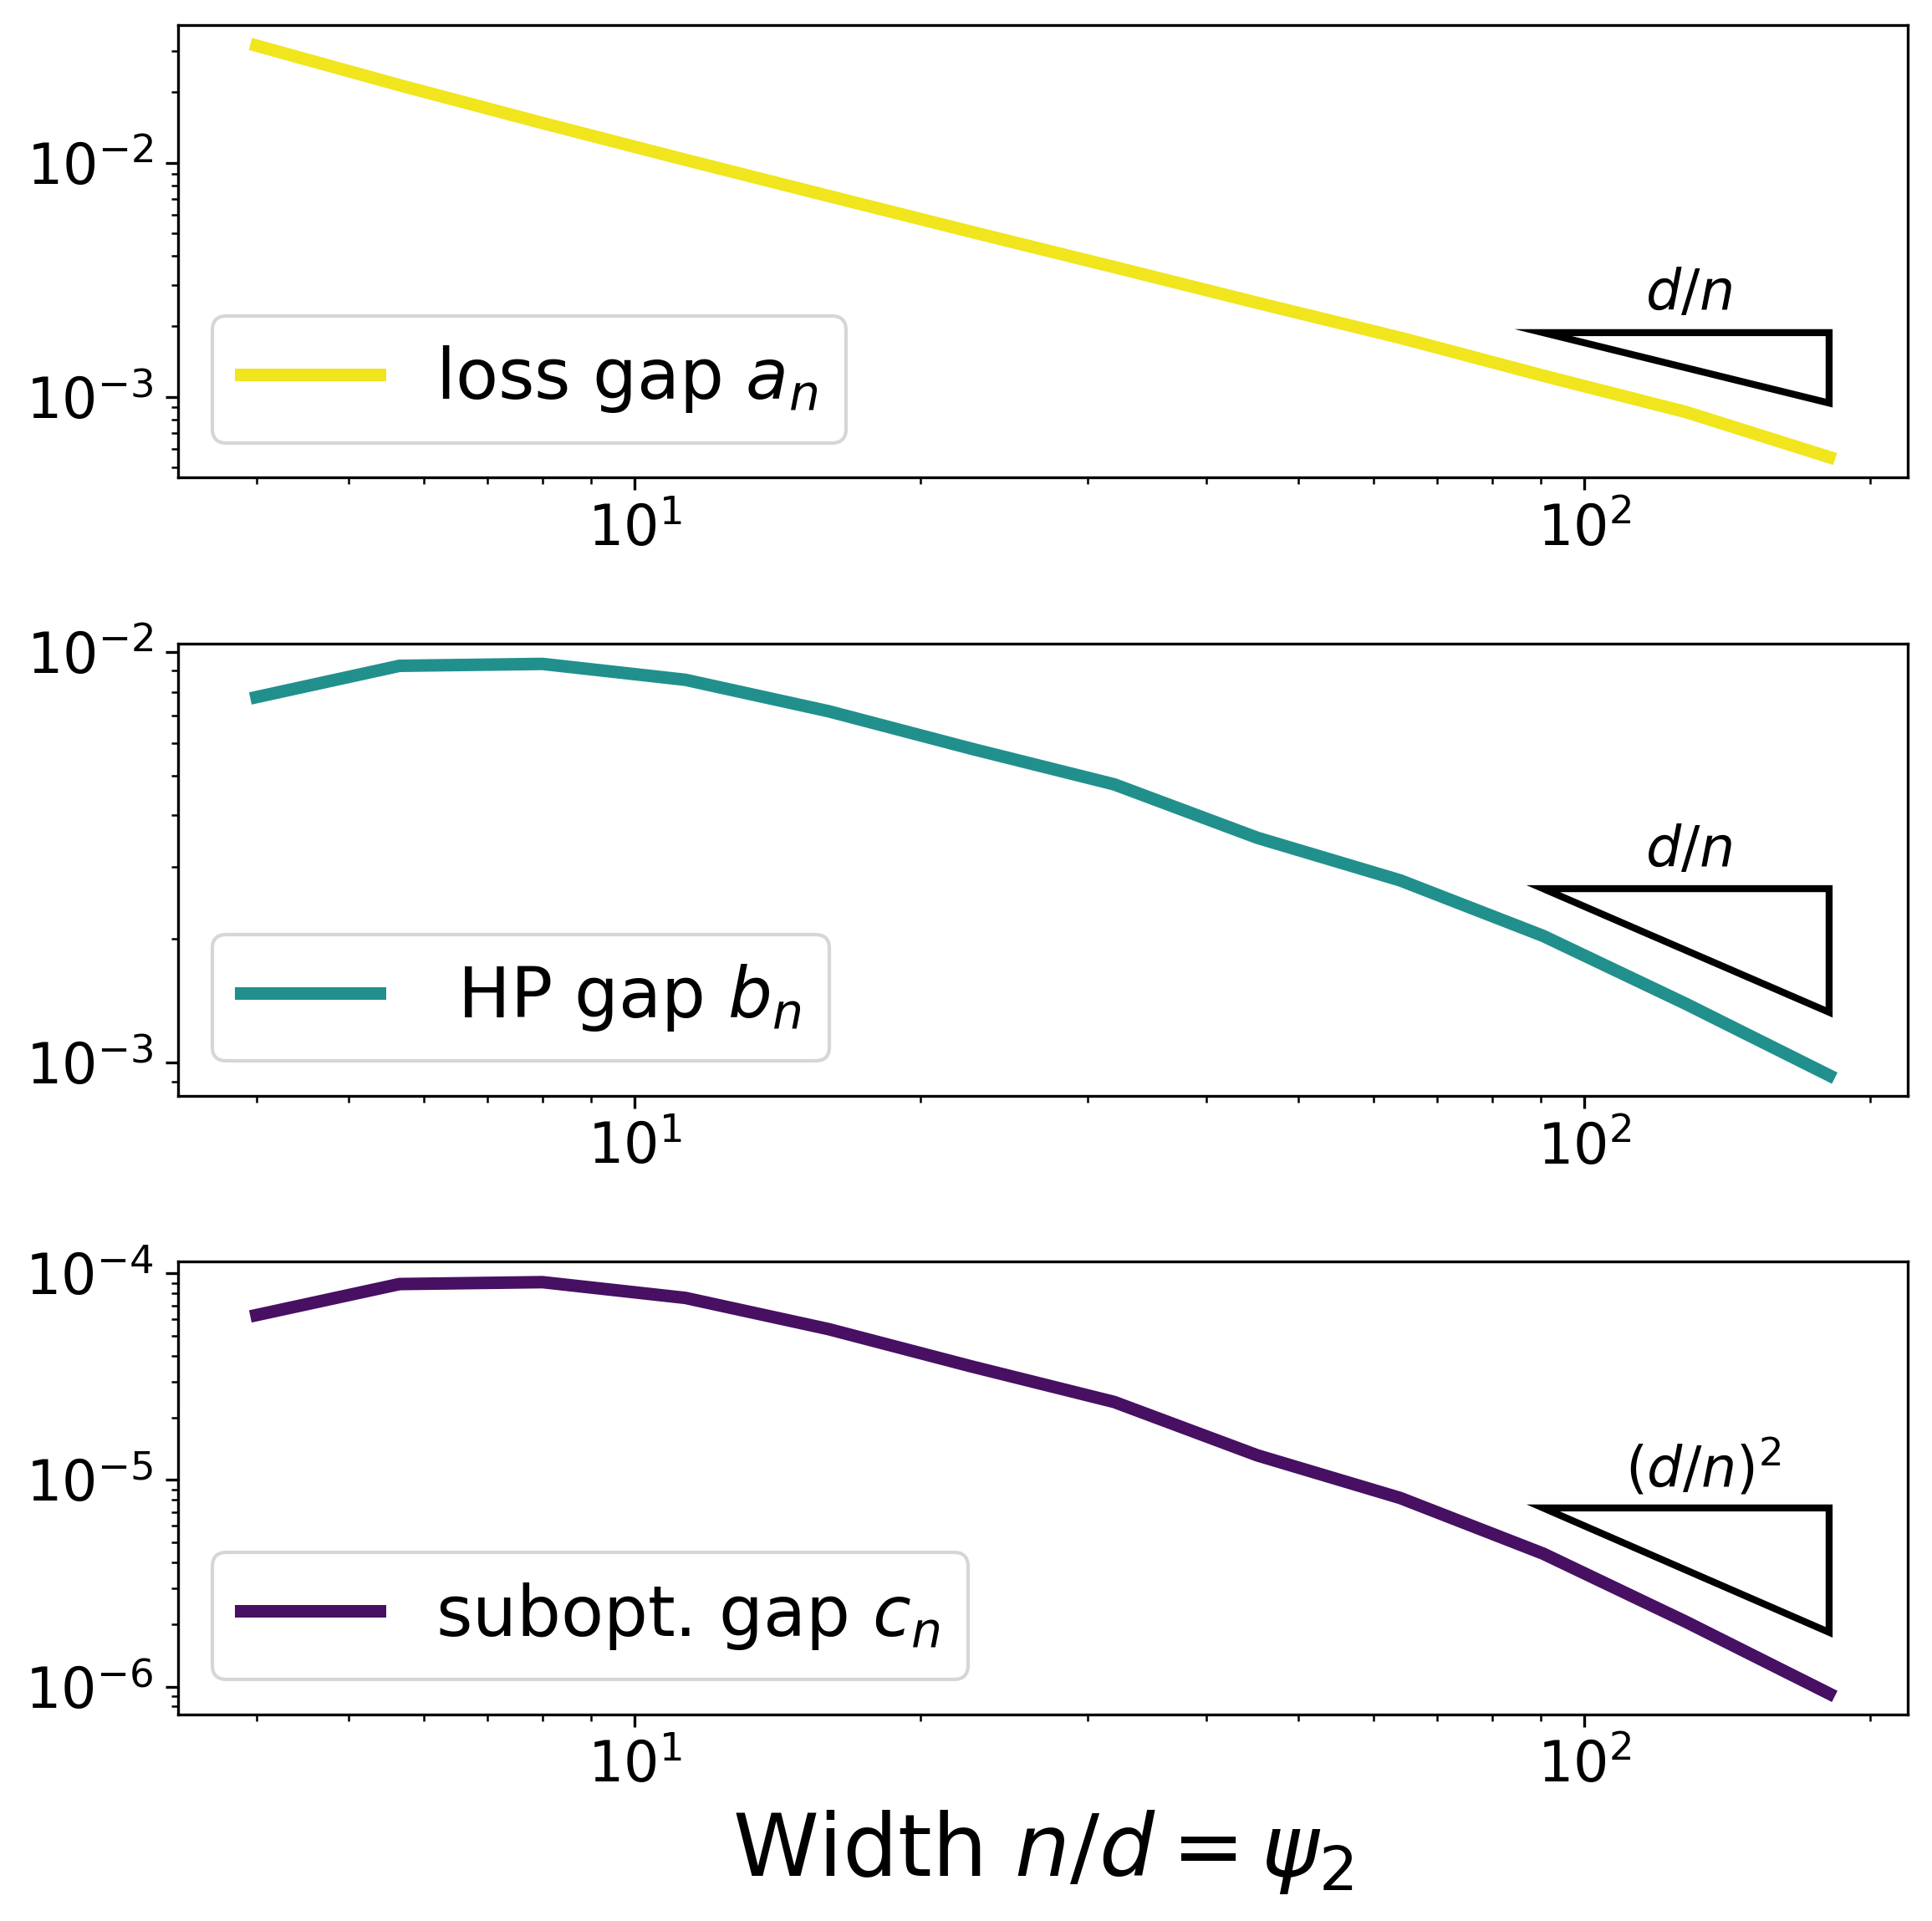
\includegraphics[height=0.72\textwidth]{figure/RFF_rate.png}} 
\end{minipage}%
% \vspace{-5mm}
\vspace{-1mm}
\end{figure}

\end{frame}  

\begin{frame}
\frametitle{Example of Slow Transfer}
\vspace{1.2mm}

{\small
\begin{itemize}\setlength\itemsep{0.25em}  
    \item \textbf{\colorbox{teal!12}{Task}: Norm Indicator Function.} 
    {\color{lightgray!60!black} $y = \mathbbm{1}\big\{\norm{\vx}_2^2 > F_{\chi_d^2}^{-1}(0.5)\big\}, ~ \text{where}\, \textstyle\vx\sim\mathcal{N}(0,\vI_d).$}\!\!\!\!\!
    \item \textbf{\colorbox{teal!12}{Model}: Two-layer ReLU network ($\mu$P)}. 
    {\color{lightgray!60!black} $f(\vx) = \sum_{i=1}^n a_i \sigma(\langle \vw_i,\vx\rangle + b_i)$.}
    \item \textbf{\colorbox{teal!12}{HP of Interest}: Adam Learning Rate $\eta$.} {\color{lightgray!60!black}Minimizing validation cross-entropy loss.}\!\!\!
\end{itemize}
}

\visible<2->{

\begin{figure}[t]
\vspace{-2mm}
\centering
\begin{minipage}[t]{0.49\linewidth}
\centering
{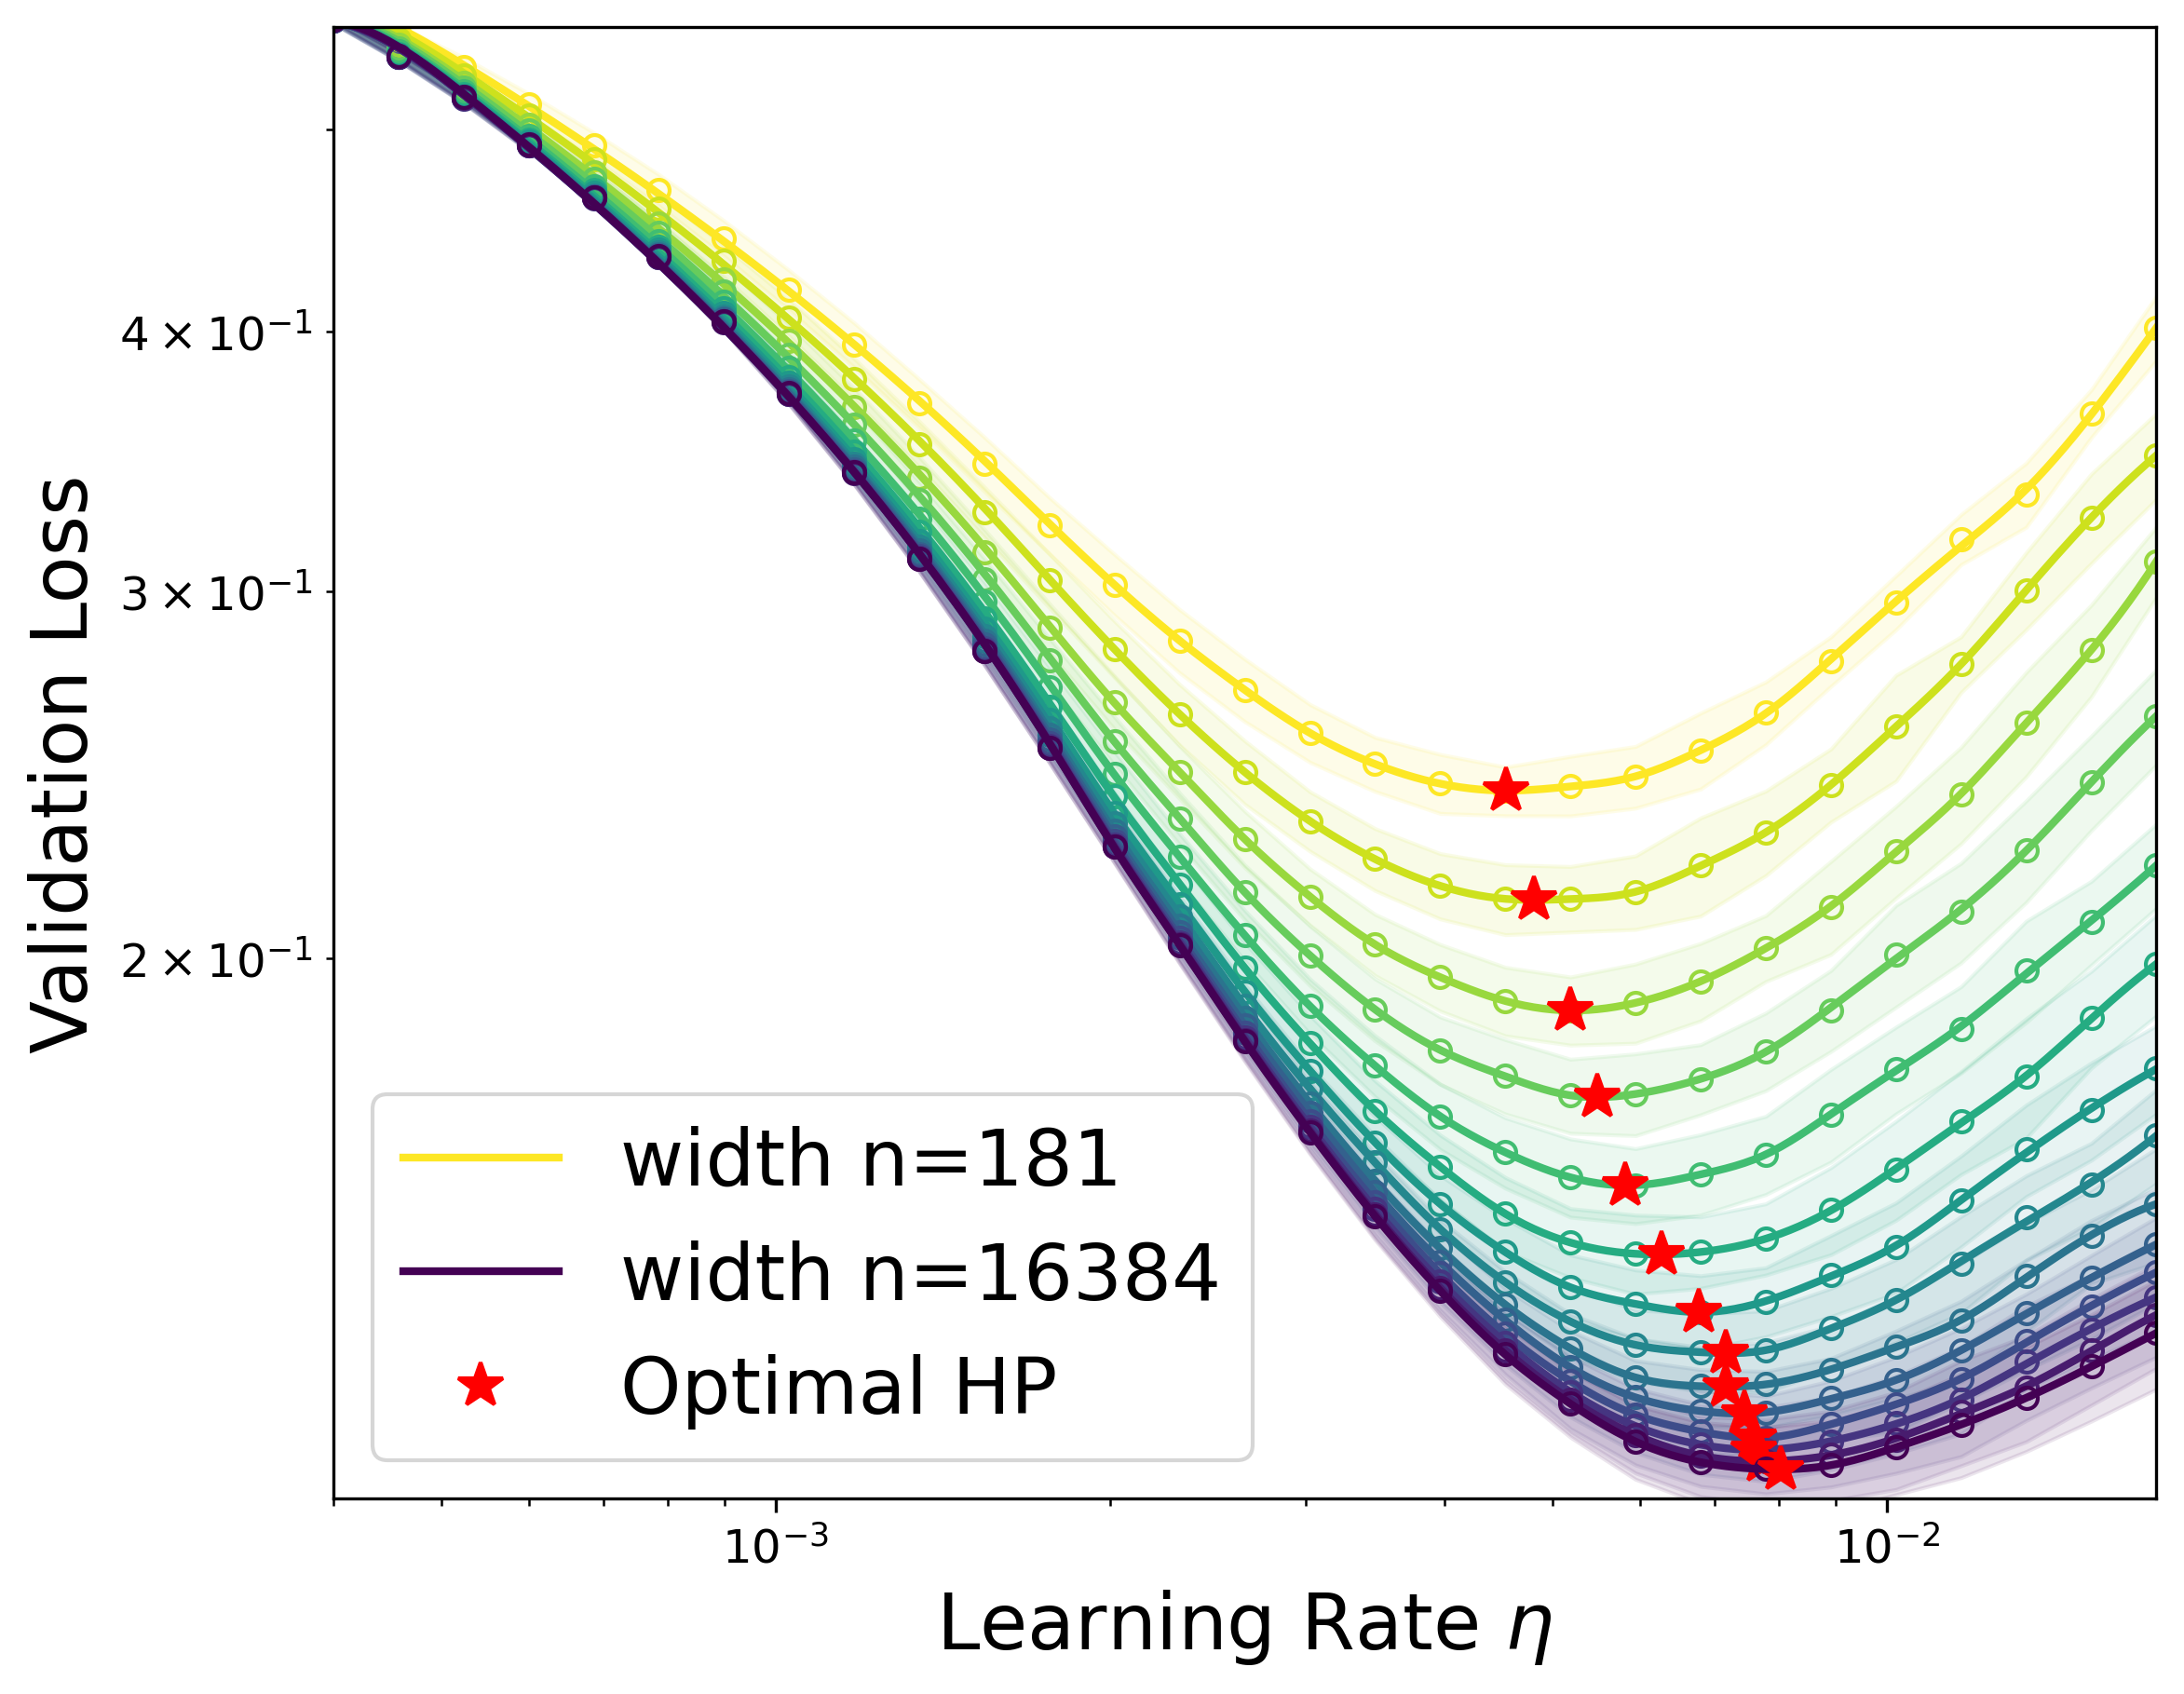
\includegraphics[height=0.69\textwidth]{figure/two_layer_ReLU_loss.png}}  
\end{minipage}%
\visible<3->{
\begin{minipage}[t]{0.49\linewidth}
\centering 
{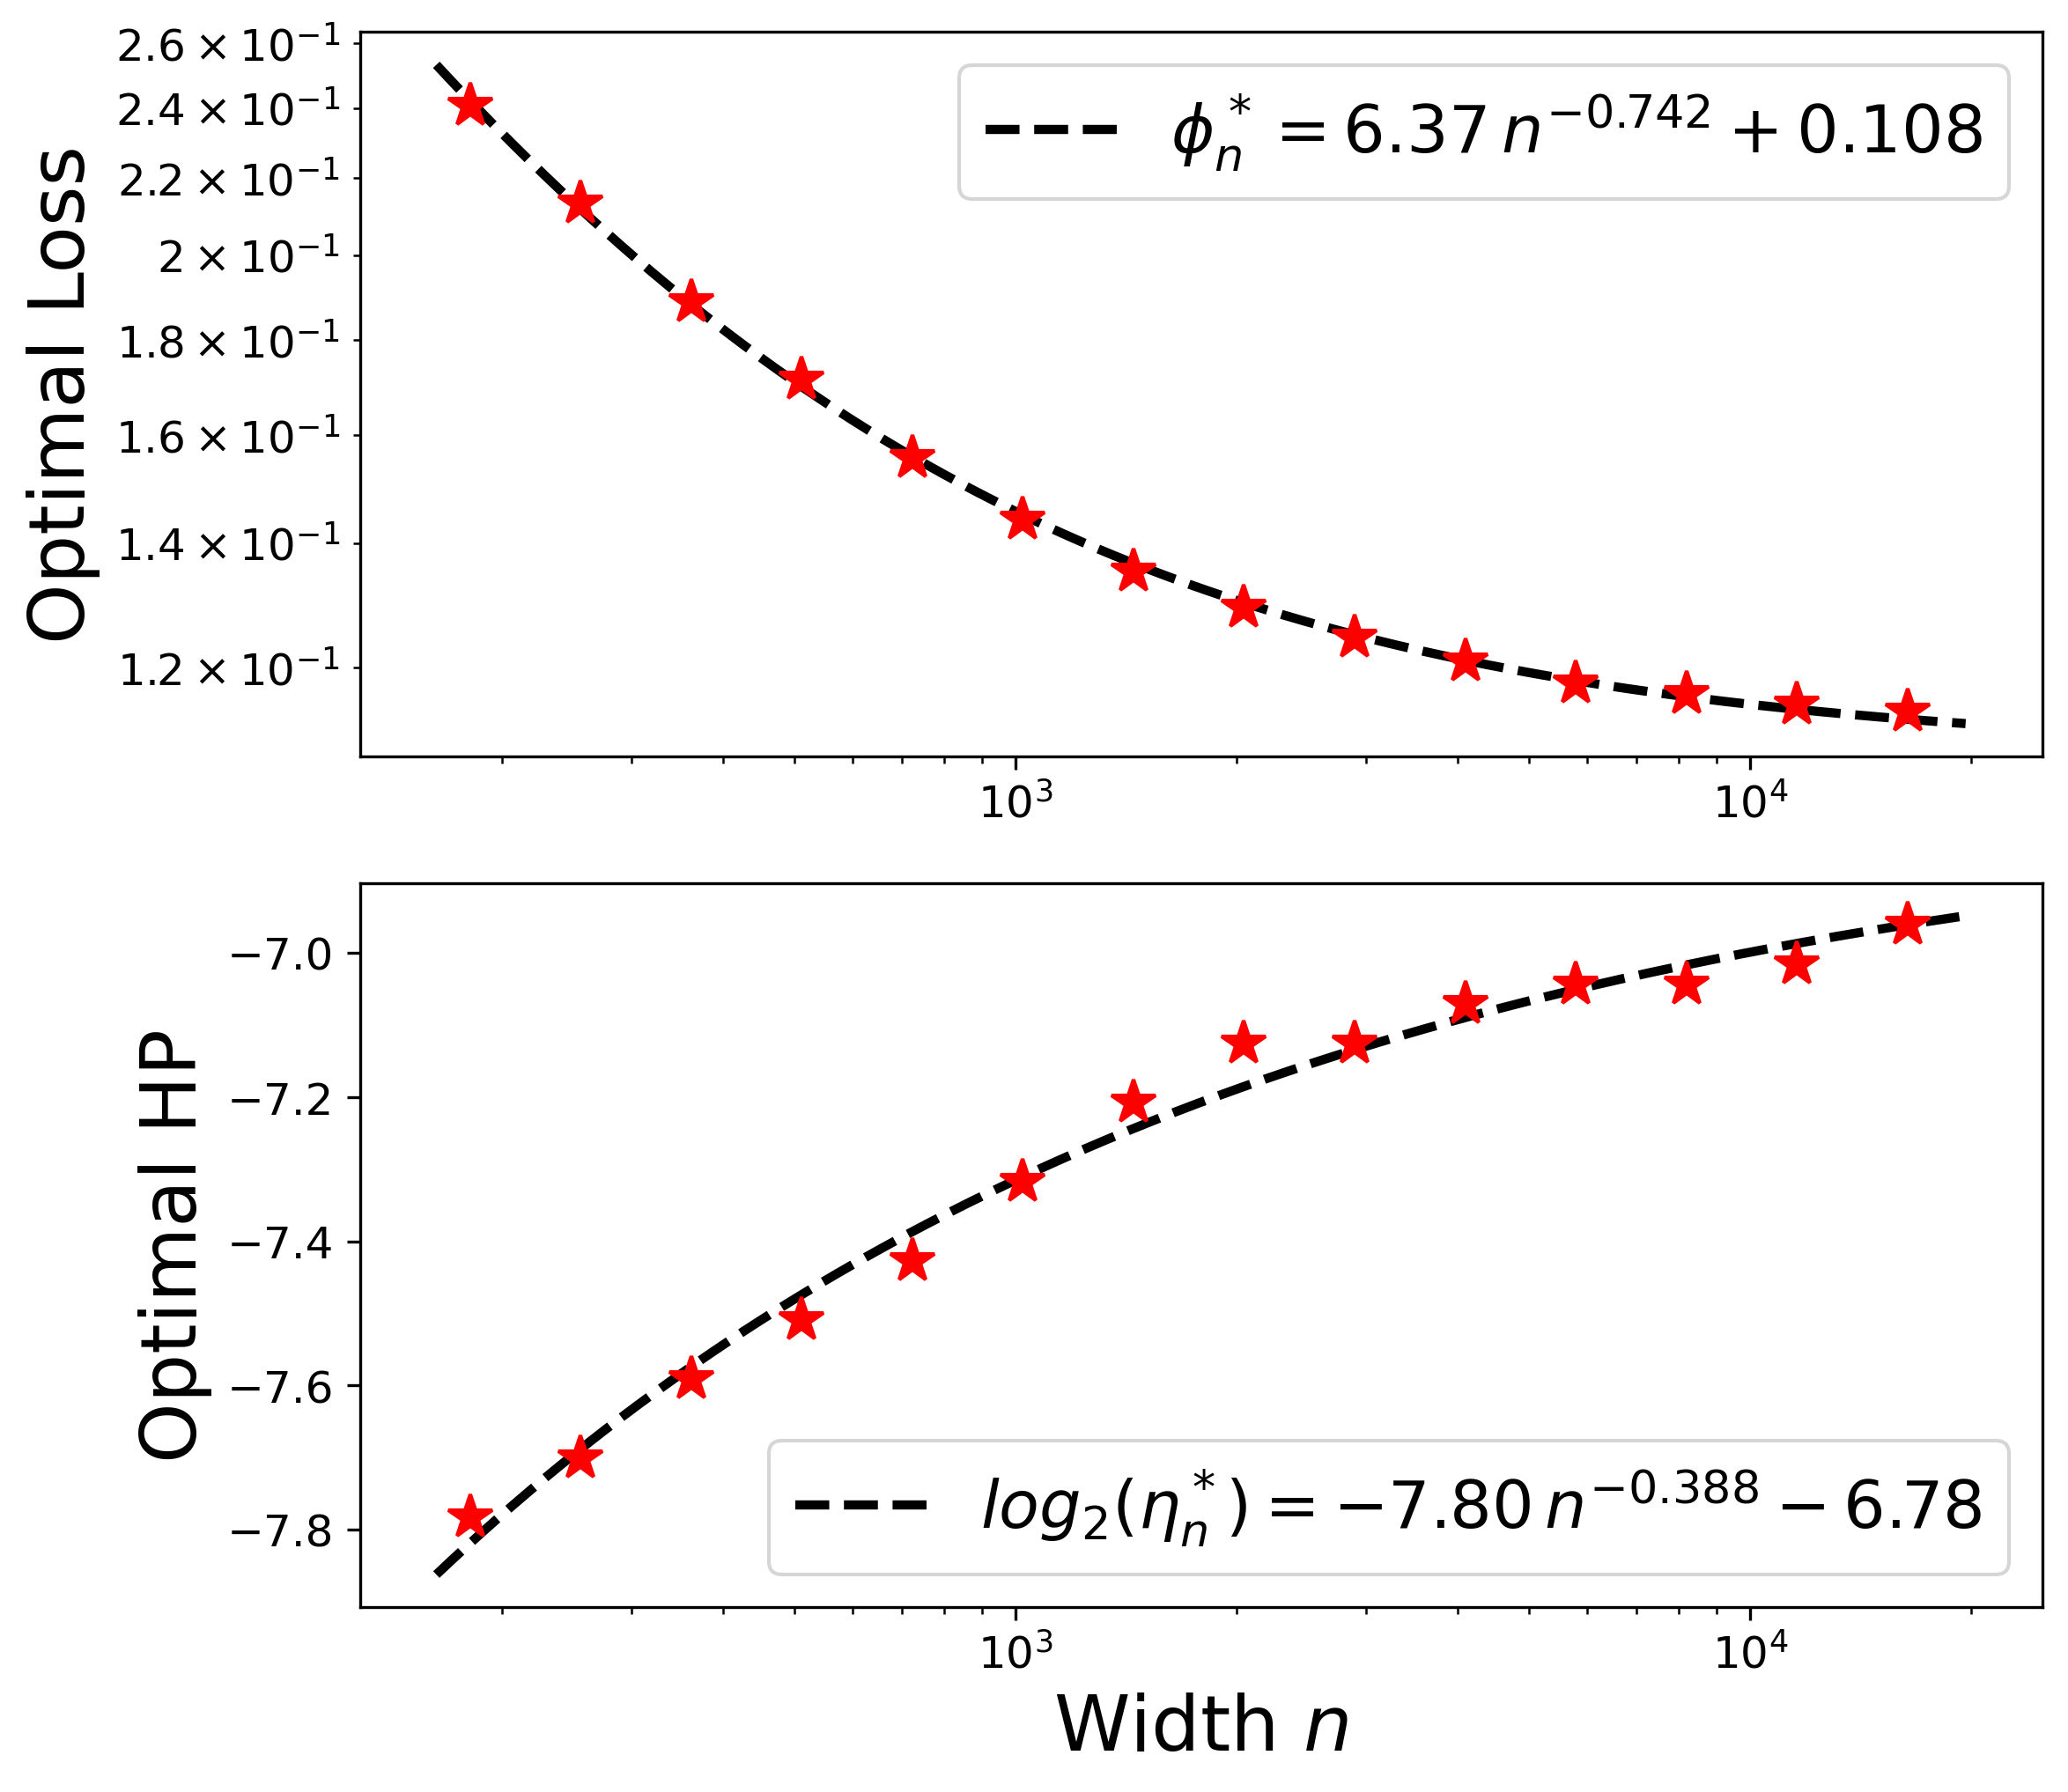
\includegraphics[height=0.69\textwidth]{figure/two_layer_ReLU_rate.png}} 
\end{minipage}%
}
% \vspace{-5mm}
\vspace{-2mm}
\end{figure}

\begin{block}{}
\begin{itemize}\small 
    \item \textbf{Left:} the optimal learning rate $\eta$ \textit{drifts towards the right} (despite $\mu$P).
    \visible<3->{\item \textbf{Right:} $b_n\approx \sqrt{a_n}$, transfer offers \textit{\color{NYUViolet}negligible computational gain} over direct tuning.} 
\end{itemize}    
\end{block}

}

\end{frame}  

\begin{frame}
\frametitle{Example of Bimodal HP}
\vspace{1.5mm}

{\small
\begin{itemize}\setlength\itemsep{0.25em}  
    \item \textbf{\colorbox{teal!12}{Task}: Gaussian multi-index model.} 
    {\color{lightgray!60!black} $y = \sqrt{\frac{d}{4k} \sum_{i=1}^k x_i^2}, \,\, \vx\sim\mathcal{N}(0,4d^{-1}\vI_d).$}
    \item \textbf{\colorbox{teal!12}{Model}: Two-layer ReLU network ($\mu$P)}. 
    {\color{lightgray!60!black} $f(\vx) = \sum_{i=1}^n a_i \sigma(\langle \vw_i,\vx\rangle + b_i)$.}
    \item \textbf{\colorbox{teal!12}{HP of Interest}: Adam Learning Rate $\eta$.} {\color{lightgray!60!black}Minimizing validation MSE loss.}\!\!\!
\end{itemize}
}

\visible<2->{

\begin{figure}[t]
\vspace{-2mm}
\centering
\begin{minipage}[t]{0.49\linewidth}
\centering
{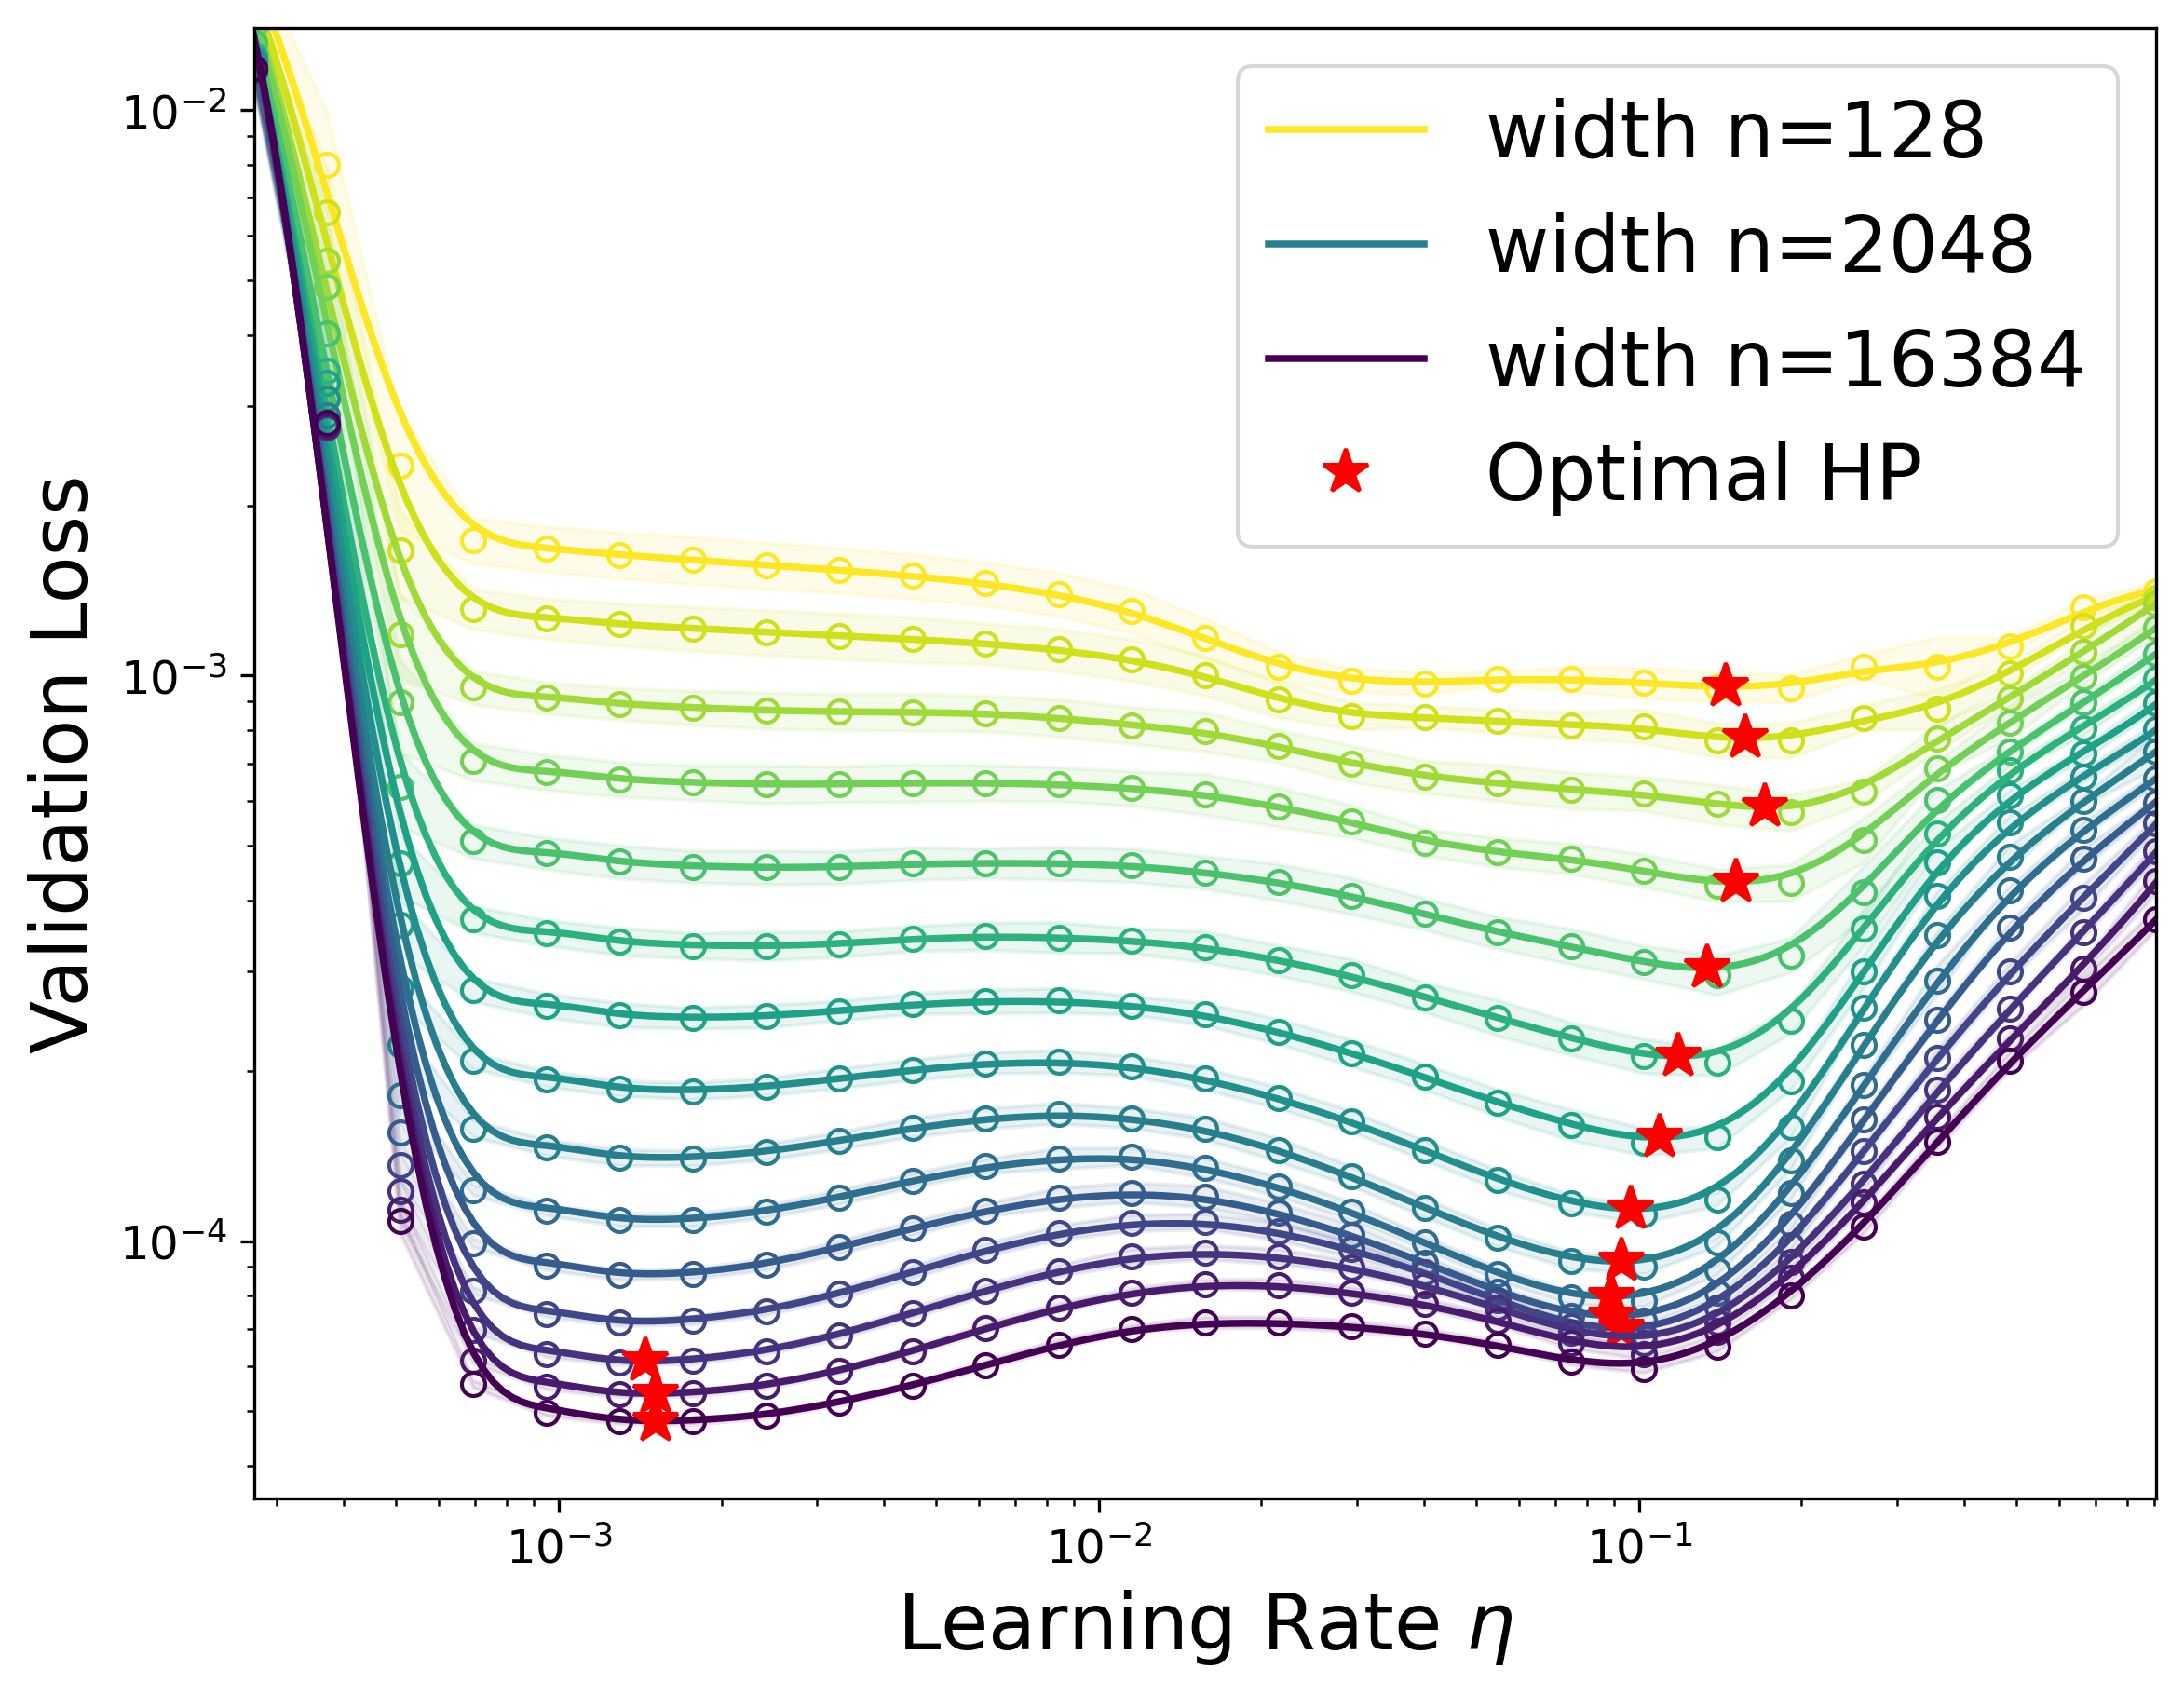
\includegraphics[height=0.69\textwidth]{figure/two_layer_ReLU_k_15_d_64_regression_loss_prefactor1.png}}  
\end{minipage}%
\visible<3->{
\begin{minipage}[t]{0.49\linewidth}
\centering 
{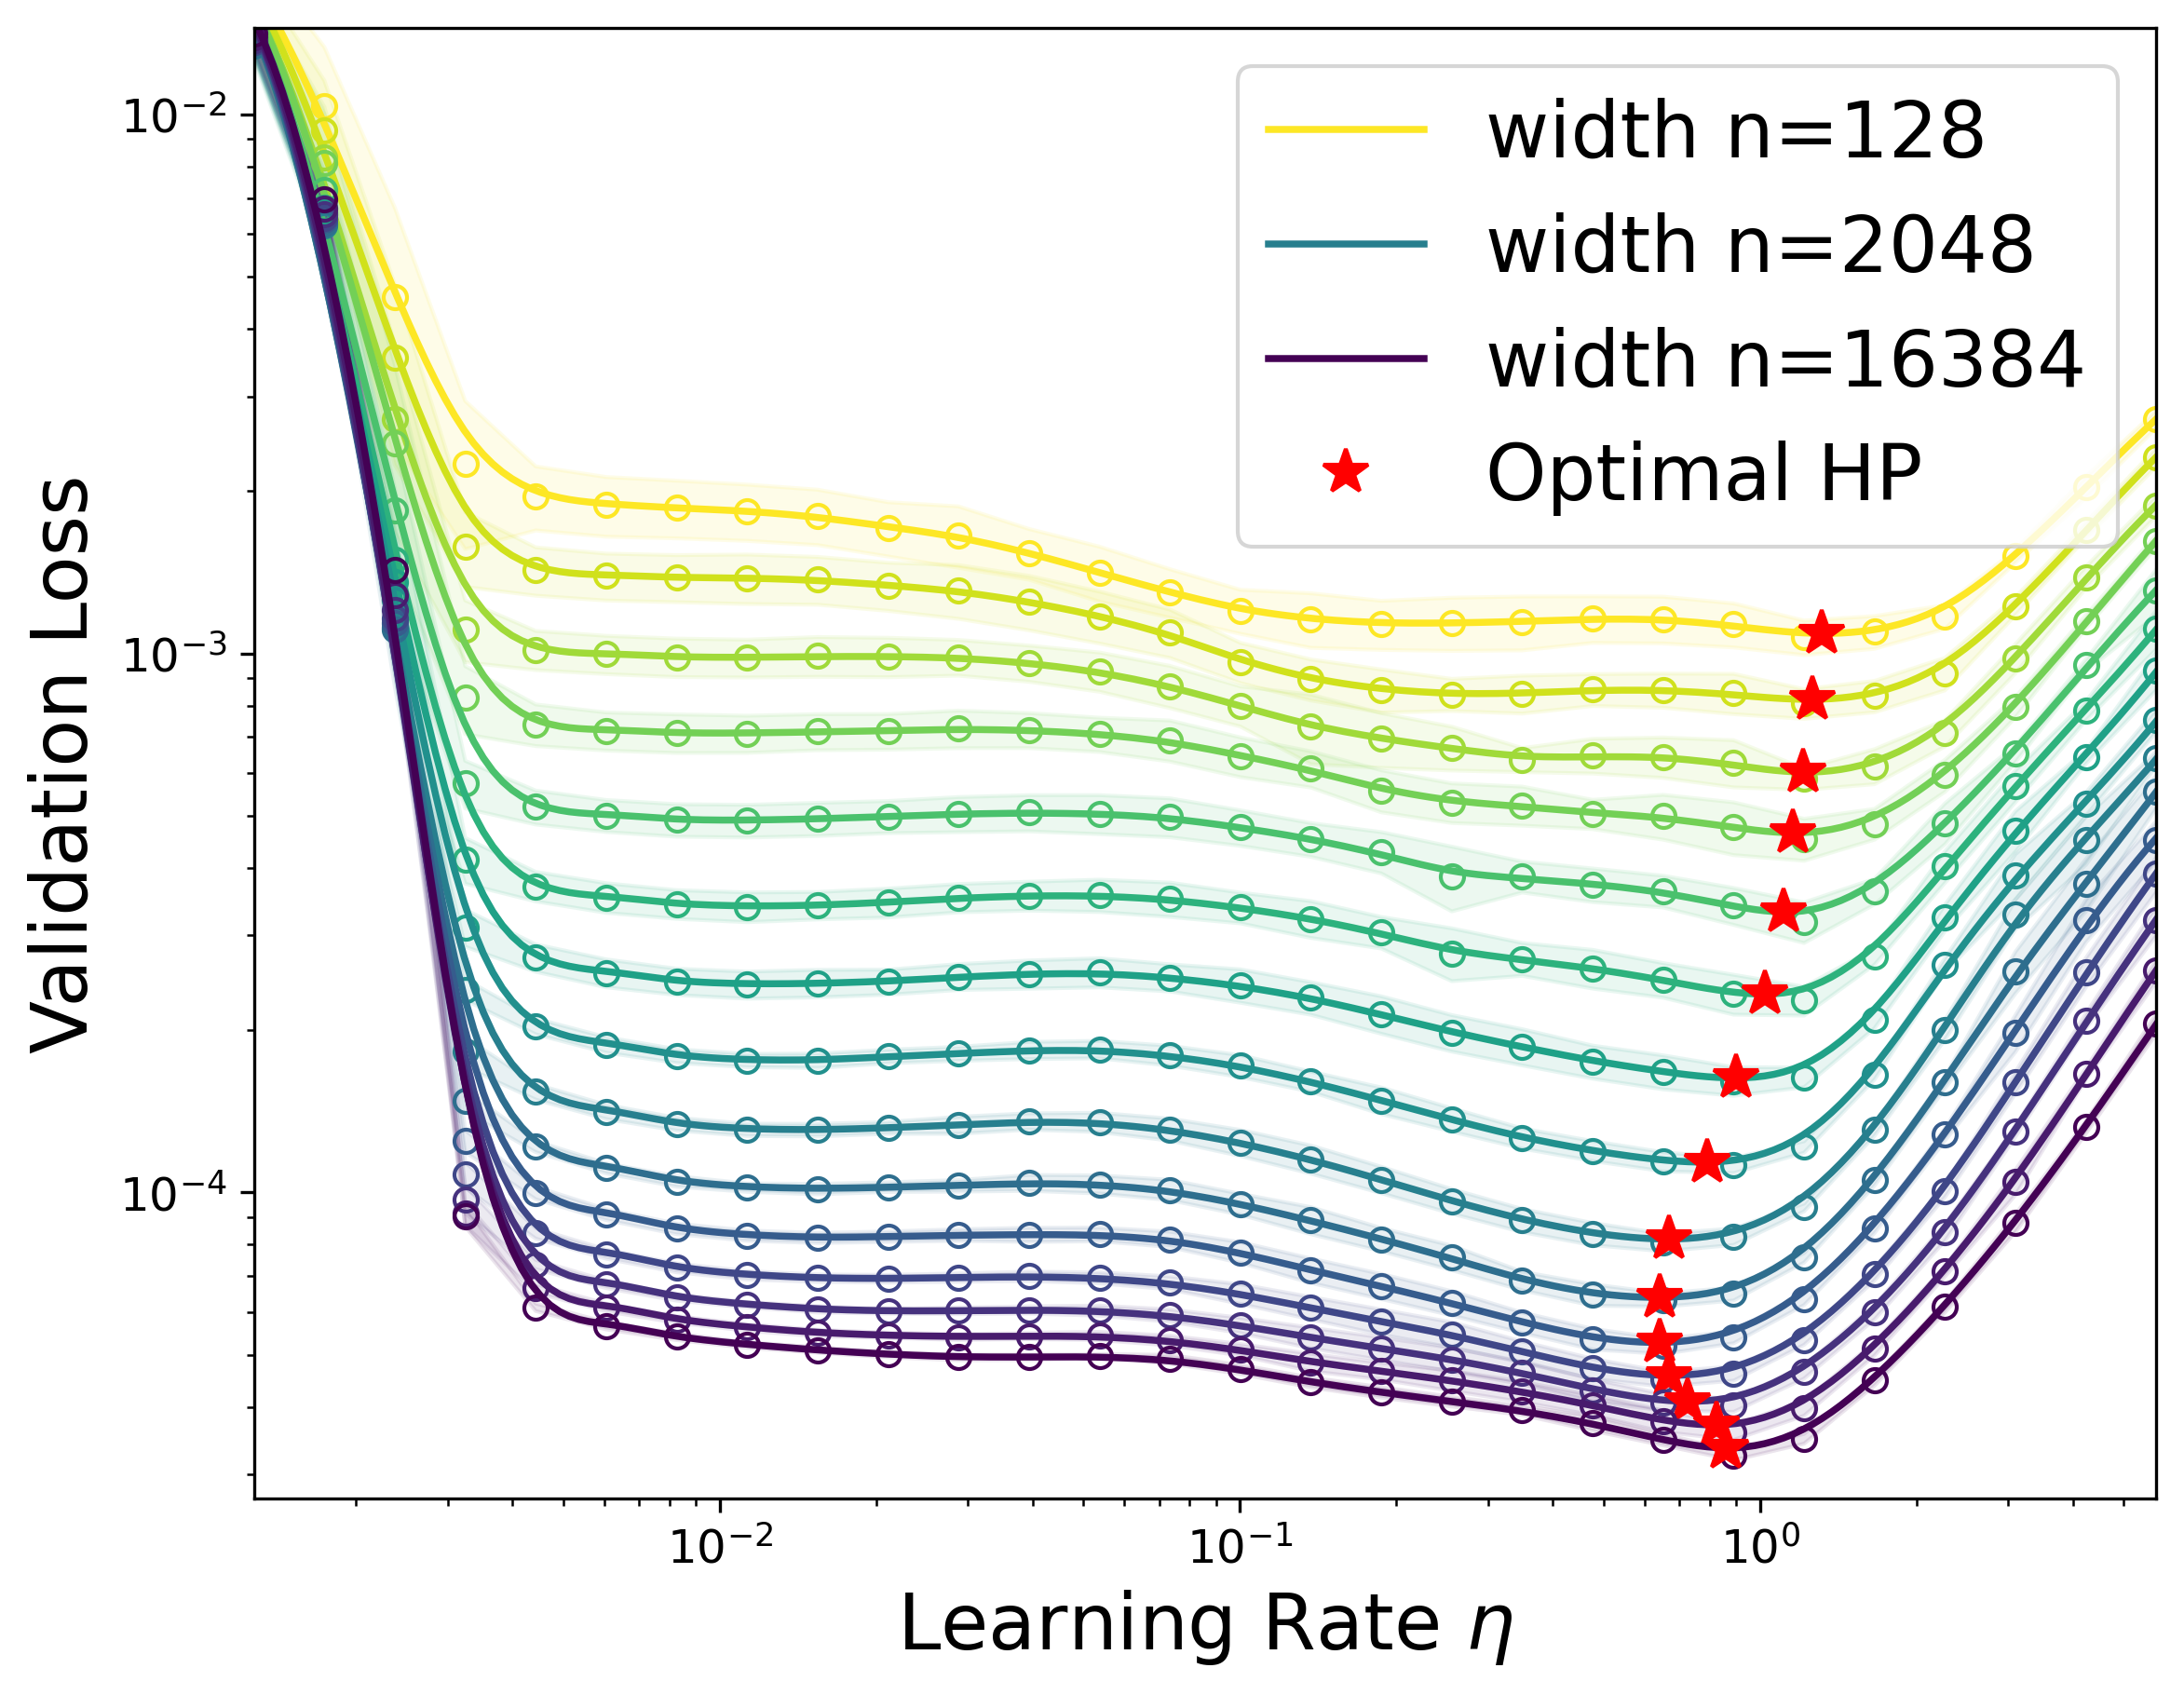
\includegraphics[height=0.69\textwidth]{figure/two_layer_ReLU_k_15_d_64_regression_loss_prefactor002.png}} 
\end{minipage}%
}
% \vspace{-5mm}
\vspace{-2mm}
\end{figure}

\begin{block}{}
\begin{itemize}\small 
    \item \textbf{Left:} default $\mu$P with \textit{same learning rate} for the first- and second-layer weights.
    \visible<3->{\item \textbf{Right:} {\color{NYUViolet}layer-wise learning rate} where second-layer learning rate is \underline{divided by $50$}.} 
\end{itemize}    
\end{block}

}

\end{frame}  

\begin{frame}
\frametitle{Low-rank Decomposition of Optimization Trajectory?}
\vspace{1.2mm}

\textbf{Question:} what structures in large neural networks enable fast HP transfer? 

{
\vspace{-1mm}
\small\color{lightgray!60!black} 
HPs depend on statistics which \textit{converge faster} than those that decide loss scaling. 
}

\pause
\vspace{2mm}

\begin{block}{Conjecture: Low-dimensional Optimization Trajectory}
The optimization trajectory can be decomposed into two parts. 
\begin{itemize}\setlength\itemsep{0.25em} 
    \item[\ding{112}] \textbf{\color{FlatironOrange2!80!black}``Spike'' component} \textit{converges rapidly with $n$}, and decides optimal HP. 
    % \begin{itemize}\color{lightgray!60!black}
    %     \item e.g., low-dimensional \textit{effective dynamics} of SGD [Ben Arous et al.~2022].
    % \end{itemize}
    \item[\ding{112}] \textbf{\color{FlatironOrange2!80!black}``Bulk'' component} improves with scale, but is \textit{less sensitive} to HP.
\end{itemize}
\end{block}

\visible<3->{
\vspace{1mm}

\parbox{0.46\linewidth}{ 

\small 

{\color{lightgray!66!black} 
Training of Llama2-type architectures with Adam on WikiText-103. 
% \\(Decomposition on \textit{EMA trajectory})
}

\vspace{1mm}

\begin{itemize}
    \item \textbf{\color{blue!80!black} ``Top-$k$'' loss} stays roughly invariant across width (dim). 
    \item \textbf{\color{red!72!black} ``Residual'' loss} improves with width.  
\end{itemize}

}
\parbox{0.53\linewidth}{
\begin{minipage}[t]{1\linewidth} 
\centering    
\vspace{-1mm}
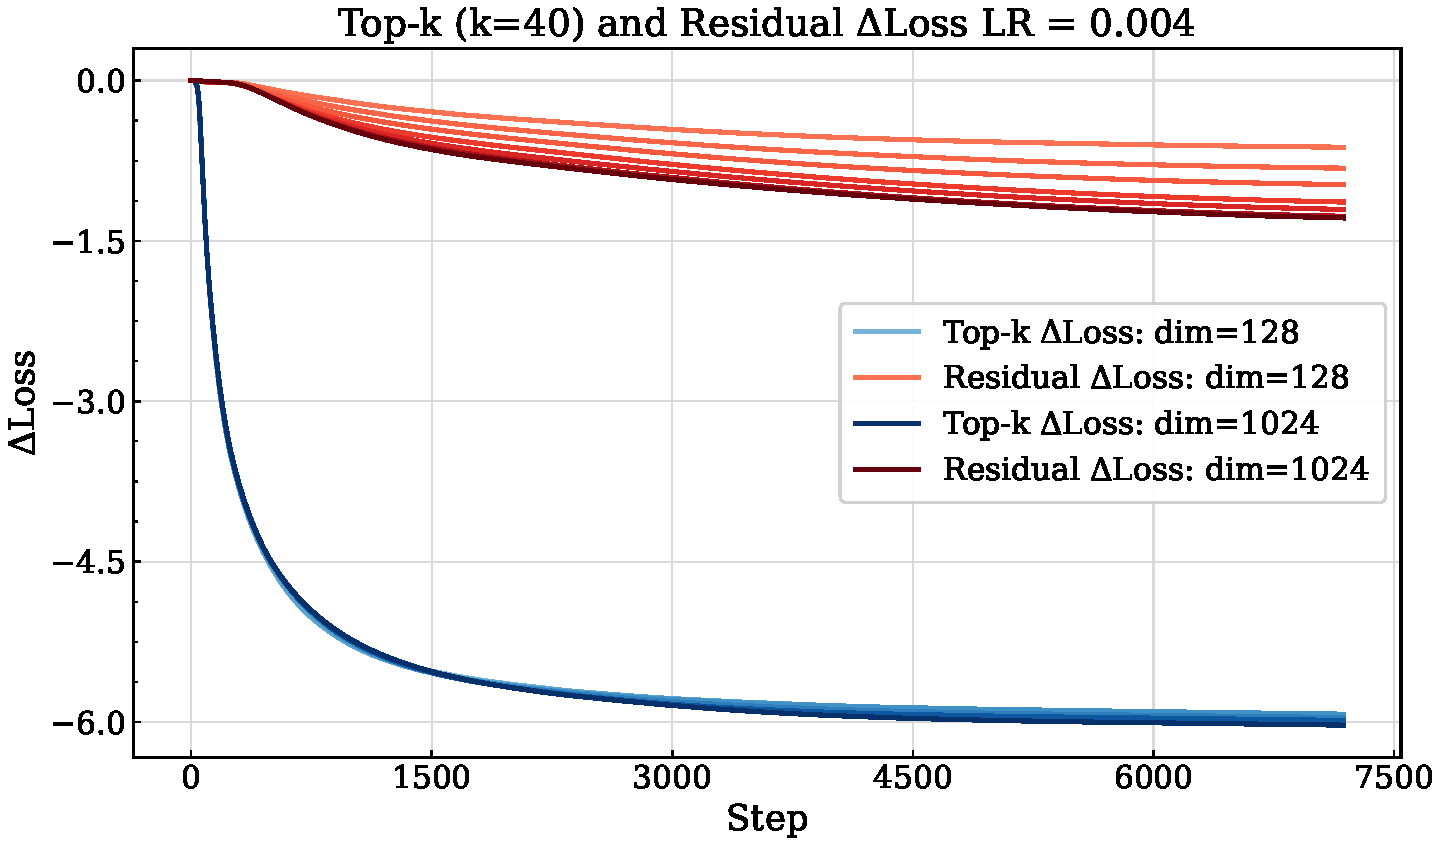
\includegraphics[height=0.58\textwidth]{figure/split_loss_over_time_lr=0.0048_ema=0.9995_seed=0_step_7185.pdf} \\  
\end{minipage}
}

}

\end{frame}  

\begin{frame}
\frametitle{Linearization and Top-$k$ Loss Decomposition}
\vspace{1.5mm}

{

\begin{block}{}
\centering
\textbf{Question:} how do we identify the ``top-$k$'' contributions of loss reduction? 
\end{block}


\small

\vspace{-1.2mm}

{\small \color{lightgray!60!black} \textbf{Rough idea:} Taylor expand optimization trajectory and track spectral properties.}

\vspace{2.5mm}
\hrule
\vspace{1.5mm}

{

\color{lightgray!60!black}

Given optimization trajectory up to time $T$:  $\vomega = (\vw_0, \ldots, \vw_T)$. 
\vspace{-0.8mm}
\begin{itemize}\setlength\itemsep{0.35em} \color{lightgray!60!black}
    \item Overall loss decrement: $\Delta \phi(\vomega) := \phi(\vw_T) - \phi(\vw_0) = \sum_{t=0}^{T-1} \delta \phi(\vw_t).$
    \item Under appropriate trajectory smoothness, 
    $\Delta \phi(\vomega) \approx \sum_{t=0}^{T-1}\langle\nabla \phi(\vw_t), \delta\vw_t\rangle$. 
\end{itemize}

}

\vspace{1mm}

\pause 

\colorbox{red!12}{\underline{\textbf{Challenge I}:}} Loss trajectory is not smooth. {\color{lightgray!60!black}(e.g., edge of stability) }

\begin{itemize}\small 
    \item[\ding{112}] \textbf{Solution:} consider \textit{\color{FlatironOrange!66!gray}time-averaged (EMA) trajectory} to smooth out oscillations. 
\end{itemize}

% \pause
\vspace{1mm}

\colorbox{red!12}{\underline{\textbf{Challenge II}:}} ``Hessian'' spectral statistics are computationally prohibitive.}

\begin{itemize}\setlength\itemsep{0.35em}\small 
    \item[\ding{112}] \textbf{Solution:} linearized loss summed over layers: $\langle\nabla \phi(\vw), \delta\vw\rangle = \sum_{\ell=1}^L \langle\nabla\vW^{(\ell)},\delta\vW^{(\ell)}\rangle$.\!\!\!\!\!\!
    \item[$\Rightarrow$] {\color{FlatironOrange!66!gray}Layer-wise SVD} gives top-$k$ components that (roughly) maximize loss decrement. 
\end{itemize}

\end{frame}  

\begin{frame}
\frametitle{Fast Transfer via Trajectory Decomposition}
\vspace{1.25mm}

\small
\begin{itemize}
\item \textbf{Setting:} Llama2-type architectures + Adam optimizer on WikiText-103.
\item \textbf{HP of interest:} Adam learning rate to minimize validation loss. 
\end{itemize}

\vspace{1.mm}


\begin{block}{}
\begin{itemize}\setlength\itemsep{0.3em}\small 
    \item<2->[\ding{112}] \textbf{Observation I:} HP transfer across width (transfer does not alter scaling law). 
    \item<3->[\ding{112}] \textbf{Observation II:} Top-$k$ loss profile almost \textit{invariant} up to $k\approx 50$. 
\end{itemize}    
\end{block}


\begin{figure}[t]
\vspace{-1mm}
\centering
\visible<2->{
\begin{minipage}[t]{0.48\linewidth}
\centering
{
\includegraphics[height=0.6\textwidth]{figure/ema_adam_lr_step_7185.pdf}}  
\end{minipage}%
}
\only<2>{
\begin{minipage}[t]{0.48\linewidth}
\centering 
{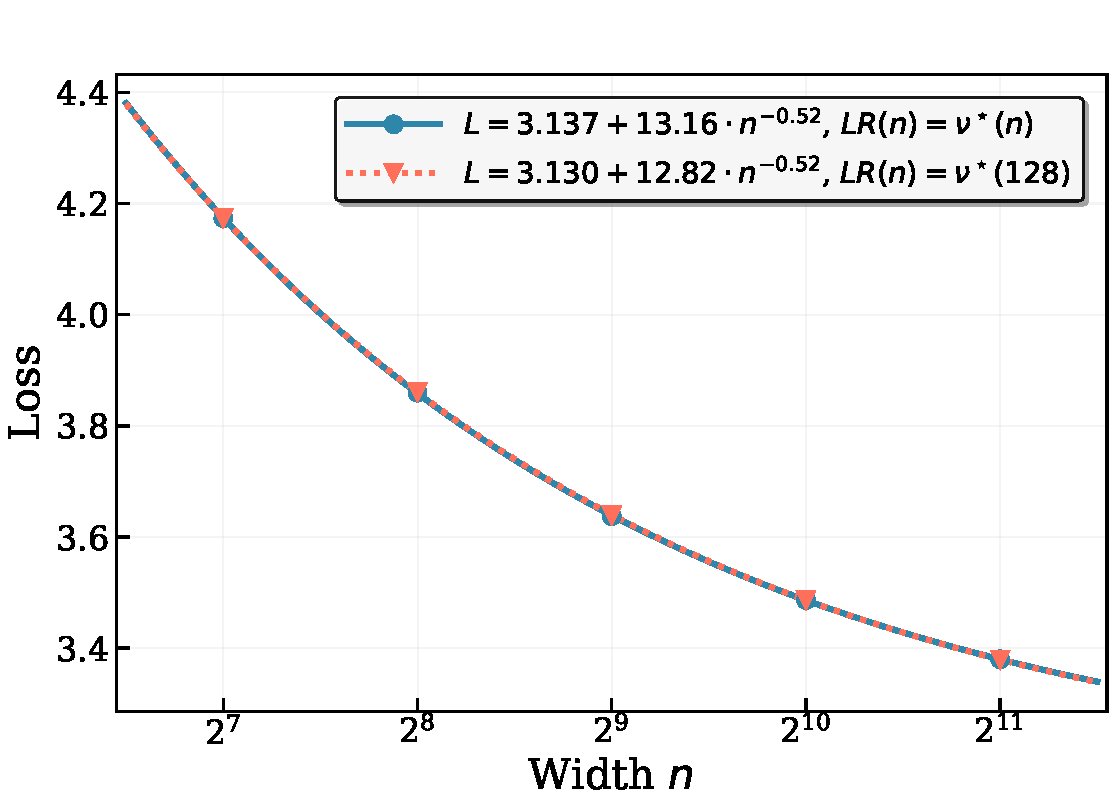
\includegraphics[height=0.6\textwidth]{figure/overlay_ema_adam_step_7185.pdf}} 
\end{minipage}%
}
\visible<3->{
\begin{minipage}[t]{0.48\linewidth}
\centering 
{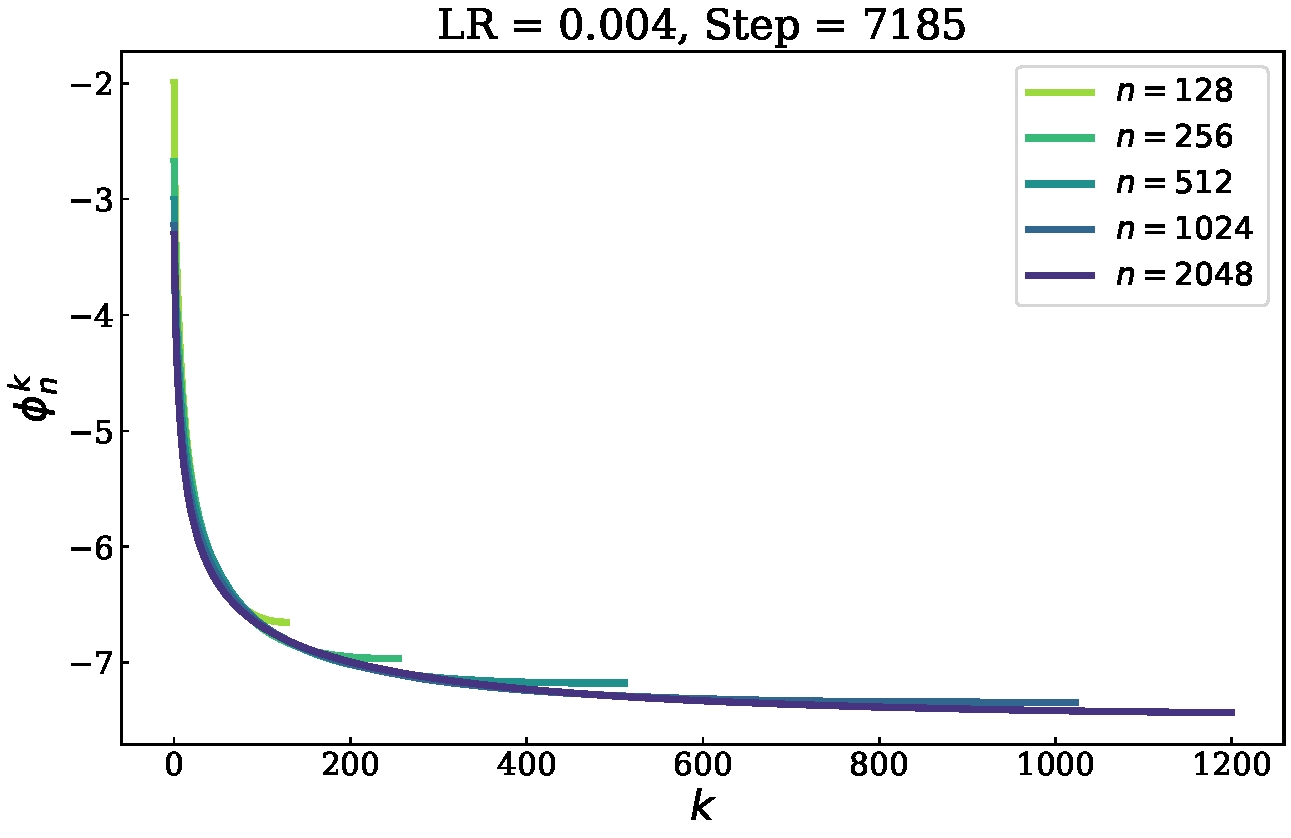
\includegraphics[height=0.6\textwidth]{figure/ema_adam_lr_topk_profile_step_7185.pdf}} 
\end{minipage}%
}
% \vspace{-5mm}
\vspace{-1mm}
\end{figure}

\visible<4>{
\begin{alertblock}{}
\small\centering
\textbf{Conjecture:} top-$k$ loss for $k\ll n$ approximately decides the optimal learning rate.
\end{alertblock}
}

\end{frame}  

\begin{frame}
\frametitle{Fast Transfer via Trajectory Decomposition}
\vspace{1.5mm}

{\small
Define $\phi^k_n$, $\phi^{-k}_n$ to be the top-$k$ and residual losses; $\vnu_n^{k*}$ is the optimal HP for $\phi^k_n$. 

}
\vspace{0.5mm}

\begin{block}{}
\textbf{\color{FlatironOrange!80!black}Conjecture} (\textit{qualitative}). There exists some chosen $k\in\N_+$ such that
\begin{itemize} 
    \item[\ding{112}] \colorbox{teal!15}{\textbf{Top-$k$ LSC.}} $\phi^k_n$ is \textit{locally strongly convex} around $\vnu_n^{k*}$. 
    \item[\ding{112}] \colorbox{teal!15}{\textbf{Top-$k$ Invariance.}} Top-$k$ loss \textit{converges rapidly}: {\color{NYUViolet}$\phi^k_n\approx \phi^k_\infty$, $\vnu_n^{k*}\approx \vnu_\infty^{k*}$}.\!\!
    \item[\ding{112}] \colorbox{teal!15}{\textbf{Residual Flatness.}} Residual loss $\phi^{-k}_n$ is \textit{sufficiently ``flat''}: {\color{NYUViolet}$\vnu_n^{k*}\approx \vnu_n^{*}$}. 
\end{itemize}    
\end{block}

\only<1>{
\begin{figure}[t]
\vspace{-1.25mm}
\centering
\begin{minipage}[t]{1\linewidth}
\centering
{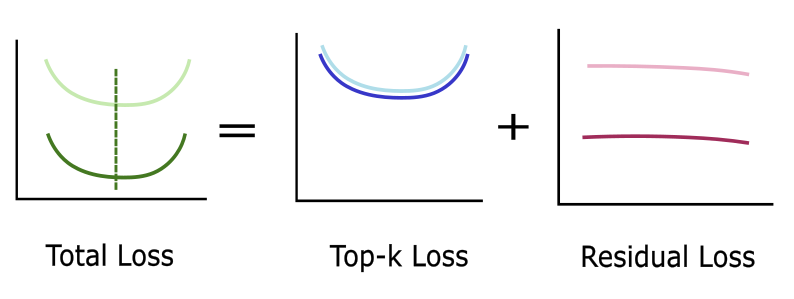
\includegraphics[width=0.8\textwidth]{screenshot/topk-illustration.png}}  
\end{minipage}%
% \vspace{-5mm}
% \vspace{-3mm}
\end{figure}
}

\visible<2->{
\begin{figure}[t]
% \vspace{-1mm}
\centering
\begin{minipage}[t]{1\linewidth}
\centering
{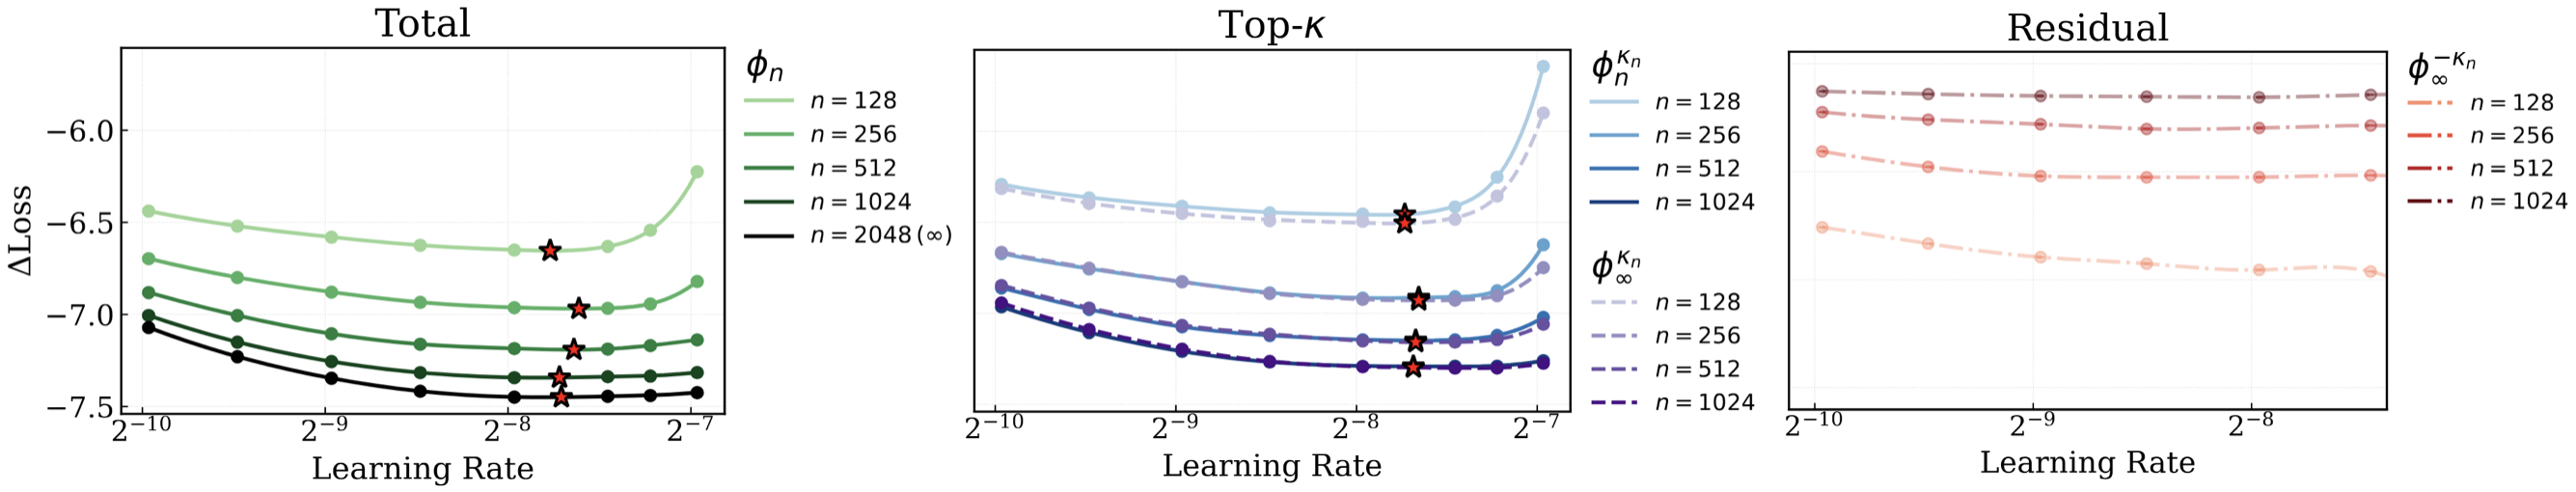
\includegraphics[width=1.02\textwidth]{figure/topk-residual.png}}  
\end{minipage}%
% \vspace{-5mm}
\vspace{-1.8mm}
\end{figure}

{\small
\begin{itemize}\color{lightgray!70!black}
\item Training of Llama2-type architectures with Adam optimizer on WikiText-103.
\item We use the largest-width model ($n=2048$) as infinite-width proxy. 
\end{itemize}
}

}

\end{frame}  

\begin{frame}
\frametitle{Matrix Preconditioning Methods?}
\vspace{1.5mm}


{
\textbf{Question:} Do different optimizers exhibit similar \textit{low-dimensional} trajectory? 

\small

\begin{itemize}
    \item MUON optimizer: $\vW_{t+1} = \vW_t - \eta \mathrm{msgn}(\nabla \cL(\vW_{t})), ~ \mathrm{msgn}(\vW) = \vU \vV^\top$.
    \item ``Whitens'' matrix-layer gradient $\Rightarrow$ promotes \textit{\color{NYUViolet}high-rank} update. 
    Per
\end{itemize}

% MUON optimizer: $\vW_{t+1} = \vW_t - \eta \mathrm{msgn}(\nabla \cL(\vW_{t})), ~ \mathrm{msgn}(\vW) = \bU \bV^\top.$

}

\vspace{0.5mm}

\begin{block}{}
\begin{itemize}\setlength\itemsep{0.4em}\small 
    \item<2->[\ding{112}] \textbf{Observation I:} HP transfer is suboptimal (transfer alters scaling law). 
    \item<3->[\ding{112}] \textbf{Observation II:} Loss profile does not exhibit clear low-dimensional invariance. 
\end{itemize}    
\end{block}


\begin{figure}[t]
% \vspace{-2mm}
\centering
\visible<2->{
\begin{minipage}[t]{0.48\linewidth}
\centering
{
\includegraphics[height=0.6\textwidth]{figure/ema_muon_lr_step_7185.pdf}}  
\end{minipage}%
}
\only<2>{
\begin{minipage}[t]{0.48\linewidth}
\centering 
{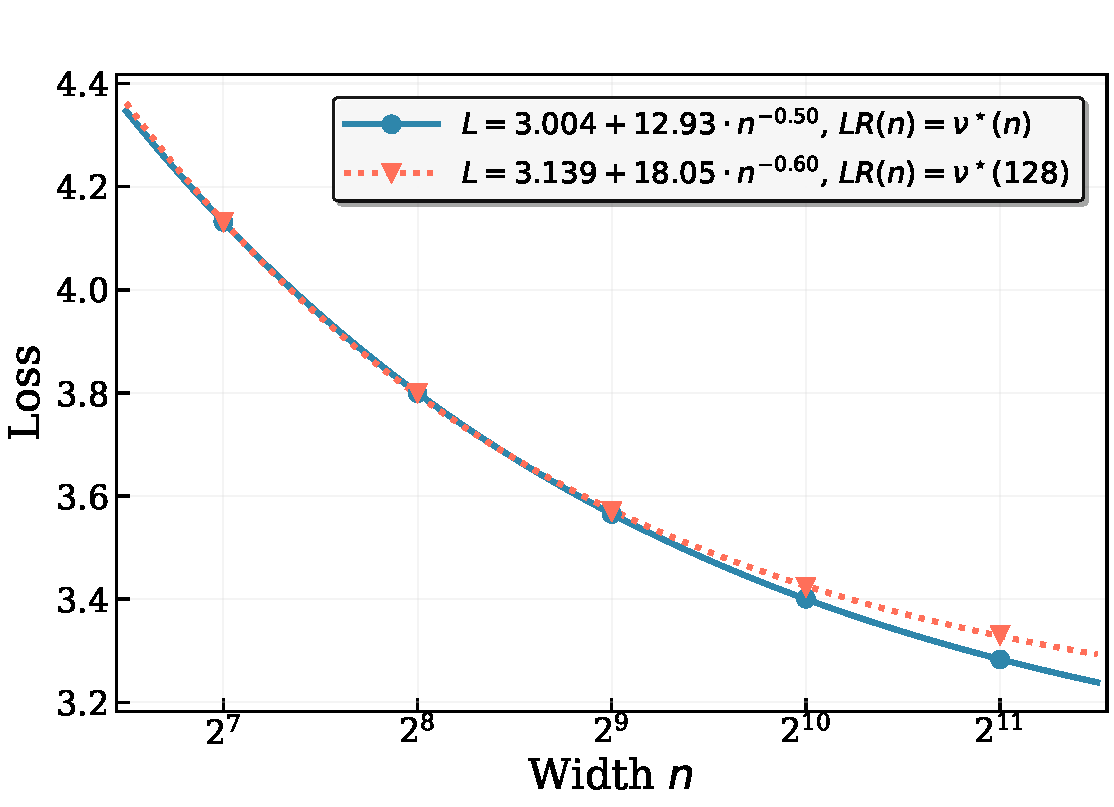
\includegraphics[height=0.6\textwidth]{figure/overlay_ema_muon_step_7185.pdf}} 
\end{minipage}%
}
\visible<3->{
\begin{minipage}[t]{0.48\linewidth}
\centering 
{
\includegraphics[height=0.6\textwidth]{figure/ema_muon_lr_topk_profile.pdf}} 
\end{minipage}%
}
% \vspace{-5mm}
% \vspace{-7mm}
\end{figure}

% \visible<4>{
% \begin{block}{}
% \small\centering
% \textbf{Open Question:} a different decomposition for matrix preconditioning updates?
% \end{block}
% }

\end{frame}  

% \begin{frame}
% \frametitle{Data-Centric View of Top-$k$ Components}
% \vspace{1.5mm}

% \end{frame}  